% REMEMBER: You must not plagiarise anything in your report. Be extremely careful.

\documentclass{l4proj}


\usepackage{minted}
\usepackage{amsmath}
\usepackage{caption,subcaption} 
\usepackage{graphicx} 
\usepackage{float}

% \usepackage[showframe]{geometry}



\begin{document}

%==============================================================================
%% METADATA
\title{Biological model for real time gaze control of a commercial security camera}
\author{Dan Cristian Cecoi}
\date{27th March 2019}

\maketitle

%==============================================================================
%% ABSTRACT
\begin{abstract}
    Every abstract follows a similar pattern. Motivate; set aims; describe work; explain results.
    \vskip 0.5em
    ``XYZ is bad. This project investigated ABC to determine if it was better. 
    ABC used XXX and YYY to implement ZZZ. This is particularly interesting as XXX and YYY have
    never been used together. It was found that  
    ABC was 20\% better than XYZ, though it caused rabies in half of subjects.''
\end{abstract}

%==============================================================================

% EDUCATION REUSE CONSENT FORM

\educationalconsent


%==============================================================================
\tableofcontents

\chapter{Introduction}
\pagenumbering{arabic} 

\section{Overview [temp]}
Deep learning technologies are at the center of the current revolution in multimedia data analysis and artificial intelligence. Over the last years, convolutional neural networks have been shown to outperform previous state-of-the-art machine learning techniques for tasks such as object detection, human pose estimation and face detection. In the majority of cases, raw images are used to train deep learning models, which carries a big penalty in training time and efficiency, with weeks or months of training time in some cases.

A solution for this problem, as demonstrated by \citet{Ozimek}, uses a biologically inspired software retina for pre-procesing of images with proven reduced memory requirements and training times without compromising on training quality. 

In this paper we present an approach to autonomously control a commercial pan-tilt-zoom security camera to capture a set of retinal transformed images used for training of Convolutional Neural Networks (CNNs).

% \section{Problem Statement}

%  \citet{RyanWong} demonstrated a portable smartphone software retina capable of automatically detecting points of interests captured by a phone's video camera. However, at present, a tool for autonomously capturing data-sets of retinal transformed images using off the shelf PTZ cameras does not exist.
%  Therefore, an autonomous mechanism for the purpose of capturing retinal transformed data sets must be developed. This will be used for the data gathering step in a training pipeline for neural networks. 
 
 



\section{Motivation [temp]}

 Biological vision systems are currently unrivaled by artificial visual systems for complex day to day tasks of an organism, such as navigating through the world, detecting dangers and identifying objects. Even the most simple tasks are still difficult for artificial systems. Due to this, biologically inspired vision systems seek to capture key aspects of the computational architecture of the brain and the sensor capabilities of the eye. Multidisciplinary inputs from other disciplines such as biology, neuroscience and cognitive science, will have a fundamental impact in the progress of computer vision. From the study of biological organisms, new types of computational paradigms can be achieved by providing a source of inspiration for new computational efficient and robust vision models.
 
 With his biologically inspired software retina, Ozimek (2017) has demonstrated an approach for pre-processing images into a data efficient form based on the human vision system. Using the retinal transformed image data was shown to drastically decrease training times and the storage requirements while not compromising on the accuracy of the deep network models.
 
 Furthermore, due to the decrease in prices of digital cameras and increase of overall quality, there is now a demand for using cheap equipment for both research and industrial computer vision applications without having to resort to using highly specialized and expensive camera systems.
 
 Our goal is to synthesise these approaches into a real-time vision pipeline which is both time and space effective and is inexpensive to set up. An application is required which can use a cheap off-the-shelf security PTZ Camera for the purpose of identifying salient regions on an object, select and explore the most important points using a saccade targeting based gaze control mechanism and collect retinal transformed data-sets with those points as the center of attention. 
 
 This work extends on existing research on the biologically inspired software retina and work done by Zhou (2018) on a graphical user interface for manually controlling a PTZ camera.
 
 
 \section{Aims [temp]}
 
There are three main objectives needed to be accomplished for the development of the autonomous capture mechanism:
 
\vspace{0.2cm}  
\begin{enumerate}
    \item The development of a non-proprietary Camera Controller component used for driving the camera.
    \item The development of an Autonomous Capture component that independently detects salient points on objects within the field of view and direct the camera towards those points.  
    \item Storing the captured data-set and demonstrate its use by loading the data into the Data Management system and training an auto-encoder with it. This will be done in collaboration with Sean Tierney, a University of Glasgow MSci student working on the Data Management application. 
    
    
\end{enumerate}



%==================================================================================================================================
\chapter{Background}

\section{Mammalian Vision System}

In the mammalian vision, light is perceived through a hemispherical layer of photoreceptor cells that convert photons into electrical signals through a series of chemical changes. The fovea, a central region of the retina where the highest density of the photosensitive cells are found, is responsible for the highest visual acuity, corresponding to 5 degrees of the visual field. Though the eye is capable of receiving visual information from a range of approximately 200 degrees, for most of that range the resolution is relatively poor due to decreasing density of the photoreceptor cells towards the peripheries of the retina. 

Once the photoreceptor cells generate the electric signals, retinal ganglion cells (RGCs) transmit the visual signal to the primary visual cortex with majority of the RGCs being connected to multiple neighbouring photoreceptor cells. This grouping of photoreceptor cells connected to each ganglion cell is called the receptive field. The receptive fields are smallest in the fovea, where each ganglion cell is only connected to individual photoreceptive cells and increase in size the further from the fovea they are located. 

By combining a small foveal region with visual attention mechanisms, biological organisms are saving on the brain's computational power and storage required to analyze a full visual scene. This has served as a motivation for numerous research into biologically inspired hardware and software retinas for computational and computer vision purposes. One such example on which this paper focuses is \citet{SumithaBalasuriya} self-organised software retina. In his work, Balasuriya explores the generation, sampling function, feature extraction and gaze control mechanisms of the software retina. 


\section{Biologically Inspired Software Retina}


Using a Self-Similar Neural Network, Balsuriya generated a receptive field tessellation with a near-uniform dense foveal region which smoothly transitions into a sparse periphery. Using this approach, the retina tessellation is created without generating local discontinuities or distortions. The positions of the Gaussian receptive fields in Balsuriya's software retina are governed by the node positions in the retina tessellation. The size of the receptive field, as is the case in the mammalian vision, scales with the distance from the center of the retina. Figure \ref{retina} shows an example of receptive field locations based on a tessellation generated using a Self-Similar Neural Network. 

% Maybe add some stuff here about how the tesselation is formed in case I need more stuff. 

Once the input image is sampled using the generated receptive fields, the intensity values at each receptive field are stored in a 1-Dimensional \textit{imagevector}. This vector is further used for the generation of the cortical and back-projected images.

\begin{figure}[H]

  \begin{subfigure}[b]{0.49\textwidth}
    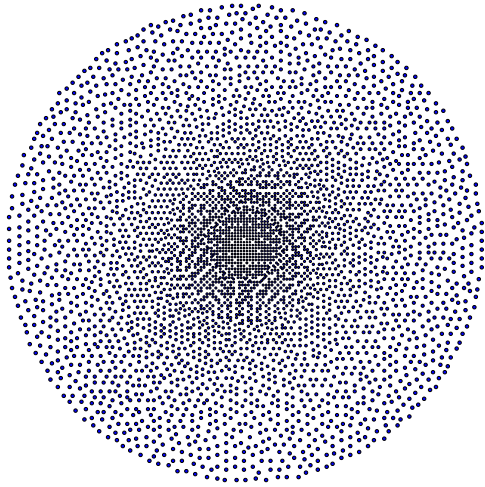
\includegraphics[width=\textwidth]{l4template-master/4ktess.png}
    \caption{Retina tesselation generated by Balasuriya}
    \label{tesselation}
  \end{subfigure}
  \begin{subfigure}[b]{0.49\textwidth}
    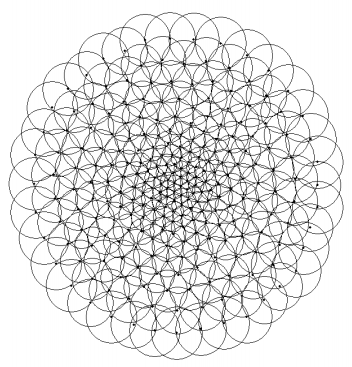
\includegraphics[width=\textwidth]{l4template-master/gaussian_rfs.png}
    \caption{Receptive fields generated from retina tesselation.}
    \label{gaussianrf}
  \end{subfigure} 
  \caption{}
  \label{retina}
 \end{figure}

\subsection{Cortical Image Generation}


Inspired by the primate visual cortex, the cortical images are data-efficient versions of the original image where the fovea is stretched out and the peripheries squashed. This is achieved by mapping the Gaussian receptive field centers to a "cortical space" and then projecting the associated imagevector intensities onto Gaussians centered on these locations. 

The cortical space is based on the work of \citet{Schwartz1977}, which proposes a model for mapping the cartesian coordinates from image space to the log-polar coordinates $(p,\theta)$, with $p$ being the distance from the origin and $\theta$ the angle about the origin.

\begin{align}
    p = log \sqrt{x^2 + y^2} \\ \nonumber
    \theta = \arctan(y/x)
\end{align}


To remove the effects of excessive densities at the periphery and of the sparseness in the foveal region, the log operator has been removed and a further work of \citet{Schwartz1980} has been adapted. In his revised approach, Schwartz adjusts the mapping with a parameter $\alpha$ while splitting the retina tesselation into two halves. Using equations \ref{hemisphereMap}, the cartesian coordinates in each half are mapped separately. This approach preserves local angles and mentains a uniform receptive field density without the introduction of noise. 


% \begin{align}
%     r = \sqrt{x^2 + y^2}
%     \label{linearlogspace}
% \end{align}


\begin{align}
    X_{left}  &= -\sqrt{(x-\alpha)^2+y^2}\\ \nonumber
    Y_{left}  &= \arctan(y/(x-\alpha)) - sign(\arctan(y/(x-\alpha)))*\pi\\ \nonumber
    X_{right} &= \sqrt{(x+\alpha)^2+y^2}\\ \nonumber
    Y_{right} &= \arctan(y/(x+\alpha)) 
    \label{hemisphereMap}
\end{align}



\subsection{Back-projected Image Generation}

The back-projected image is used as an aid to visualize the responses of the space-variant sampling allowing to examine the sharpness and the artifacts generated by the retinal sampling. To create the back-projected image, every Gaussian receptive field is scaled by its corresponding intensity values in the imagevector and is back-projected onto the original image plane. The back-projected image has information only from the retinas field of view with the rest of the image being discarded. In figure \ref{backprojected} a high resolution center corresponding to the fovea and a lower resultion periphery can be observed. 


\begin{figure}[H]

  \begin{subfigure}[b]{0.5\textwidth}
    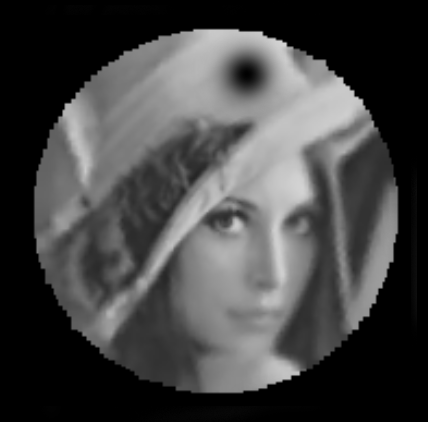
\includegraphics[width=\textwidth]{l4template-master/images/back2.png}
    \caption{Back-projected image.}
    \label{backprojected}
  \end{subfigure}
  \begin{subfigure}[b]{0.5\textwidth}
    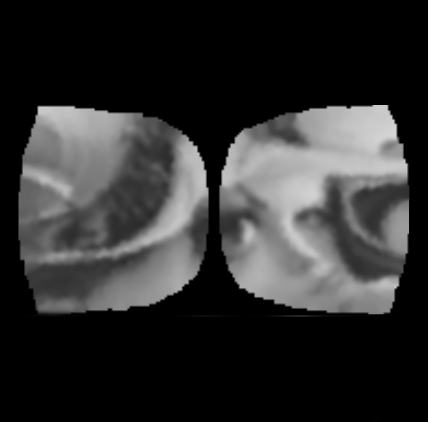
\includegraphics[width=\textwidth]{l4template-master/images/cort_lena2.png}
    \caption{Cortical image.}
    \label{cortical}
  \end{subfigure} 
  \caption{}
  \label{retina}
 \end{figure}





% ================================================================
\section{Local Feature Detection}



Image local feature extraction is a dimensionality reduction technique where the resultant information provides a low dimensional description of the image contents. Local image features can be defined as a specific pattern that is unique to its immediately close pixels. These patterns are generally associated with a change of an image property or several properties simultaneously such as intensity, colour or texture. Local features are generally points but can be corners or blobs \citep{Tinne08}. These points serve as anchors whose neighbourhoods are represented by computed feature vectors. 

Local feature extraction is the most used low-level visual representation due to robustness to occlusion and clutter, their distinctiveness, repeatability and efficiency with achievable real-time performance. They can be used in applications such as image alignment, object recognition and motion tracking.   


\subsection{Scale Invariant Feature Transform}

A wide variety of feature description and detections algorithms have been proposed in literature. One of the most robust and scale-invariant feature detectors with high repeatability is Lowe's \textit{Scale Invariant Feature Transform} (SIFT). SIFT algorithm has four main steps:





\begin{enumerate}
  \item Scale Space Extrema Detection
  \item Key point Localization
  \item Orientation Assignment
  \item Description Generation 
\end{enumerate}

\hspace{1pt}





In order to identify interest points that are scale and orientation invariant, locations and scales that can be repeatably assigned under differing views of the same subject must be identified.  To achieve this, the scale space is separated into octaves and in each octave the initial image is repeatedly convolved with Gaussians to produce a set of scale space images. To find local extrema, each level of the pyramid has its adjacent Gaussians subtracted to produce a \textit{Difference of Gaussians} (DoG). 

To accurately locate interest points, key point candidates are localised and refined by using
a Taylor series expansion of the scale space to get a more accurate location of extrema. The
intensity at these extrema is compared to a contrast threshold value, and if it's lower the
extrema is rejected. However, because the DoG function has a higher response along edges,
rejecting only key points with low contrast is not sufficient and the edge responses need to be removed as well. This is achieved by computing a 2x2 Hessian matrix, \textit{H}, at the location and scale of the keypoint, from which the principal curvature can be calculated. A poorly defined peak will have a large principal curvature across the edge but a small one in the
perpendicular direction. The eigenvalues of H are proportional to the principal curvatures of
the scale space function. Fortunately, it is not necessary to directly compute the eigenvalues
as we are only interested in the ratio between the largest magnitude eigenvalue and the
smaller magnitude eigenvalue. This ratio is compared with a threshold, \textit{r}, discarding the
keypoints whose ratio of principle curvatures is over that threshold \citep{Lowe04}.

\begin{figure}[ht]
    \centering
    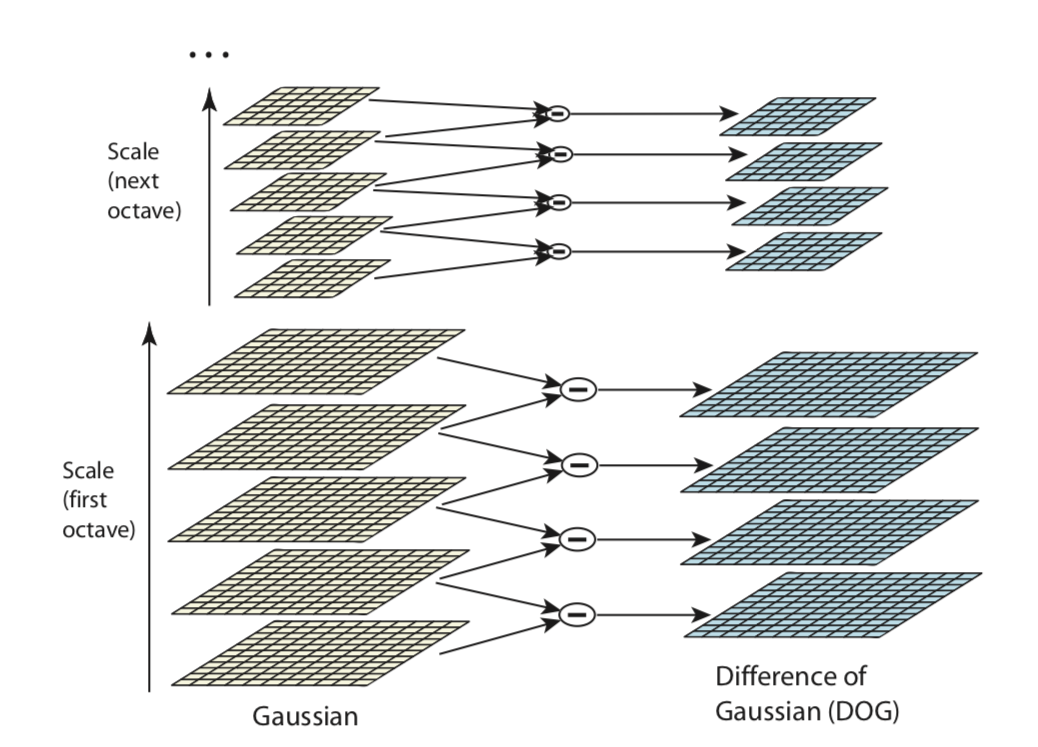
\includegraphics[width=0.8\textwidth]{l4template-master/images/gaussianPyramid.png}
    \caption{Each octave of the scale space is repeatedly convolved with Gaussians to produce the scale space images on the left. To produce the difference-of-Gaussian shown on the right, adjacent Gaussian images are subtracted. After each octave, the Gaussian image is down-sampled by a factor of 2, and the process repeated \citep{Lowe04}.}
    \label{gaussianpyramid}
\end{figure}

Orientation assignment is achieved by creating a orientation histogram of local gradient directions around the keypoint depending on the scale. The highest peak in the orientation histogram corresponds to the dominant direction of the key point.

\begin{figure}[ht]
    \centering
    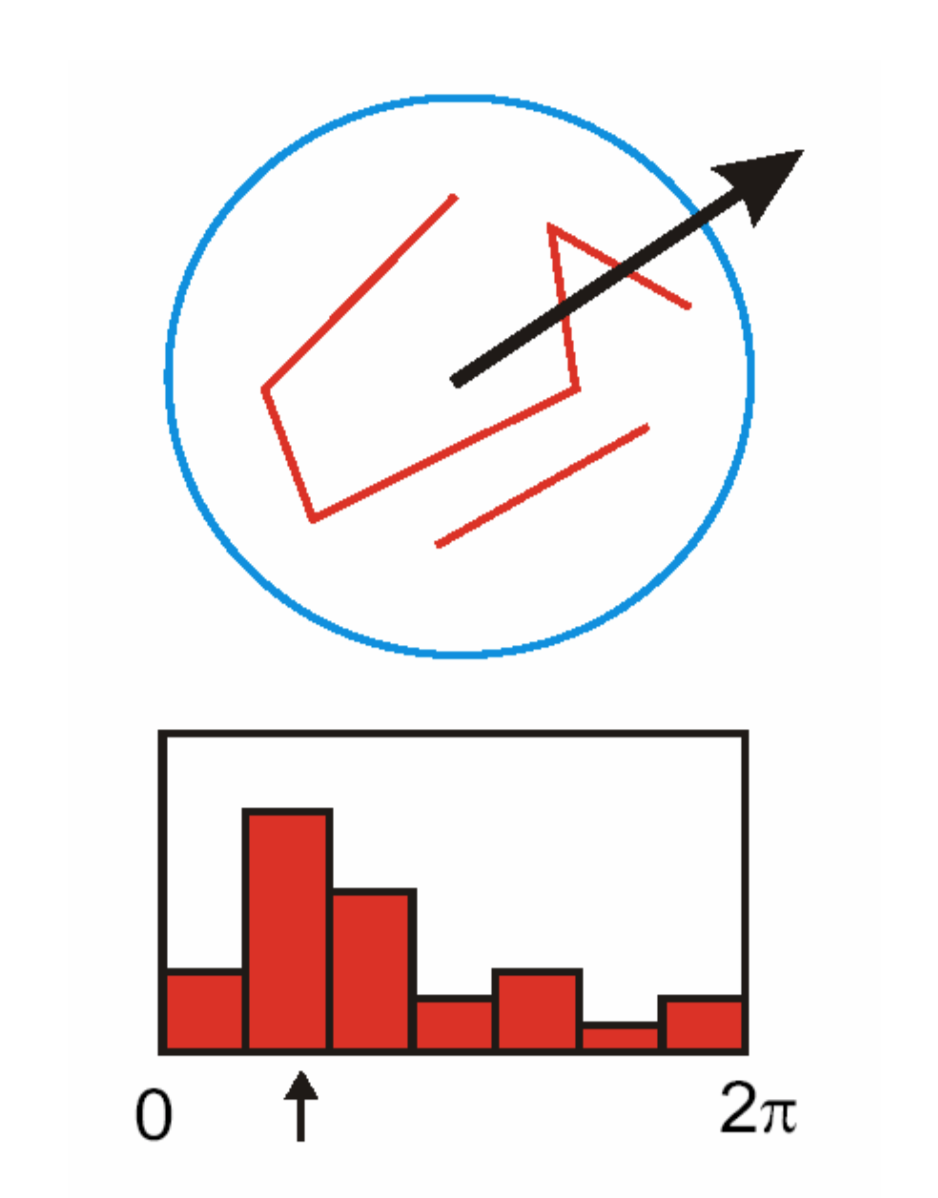
\includegraphics[width=0.3\textwidth]{l4template-master/images/orientationAssignment.png}
    \caption{Orientation Assignment by local gradient direction. \citep{Lowe04}}
    \label{orientationassignment}
\end{figure}

In the final step of the algorithm, the keypoint descriptor is created.  A 16-by-16 neighborhood around the keypoint is taken and subdivided into 4-by-4 sub regions. A orientation histogram is created over these sub regions by evaluating the magnitude of gradients in eight directions. All the orientation histograms are combined together into a 128 dimensional SIFT point descriptor. In addition to this, the feature vector is normalized in order to achieve robustness against illumination changes. 

\begin{figure}[ht]
    \centering
    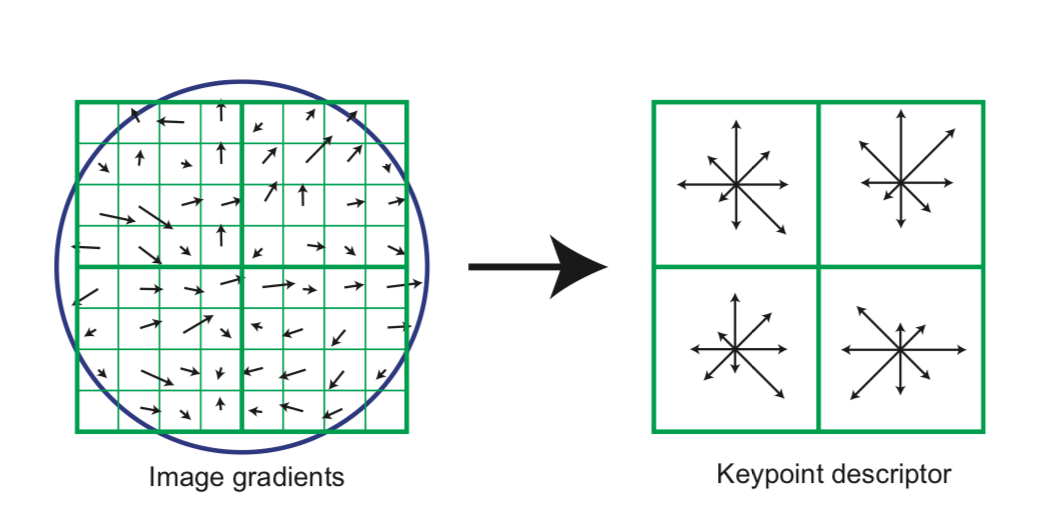
\includegraphics[width=0.7\textwidth]{l4template-master/images/keypointDescriptor.png}
    \caption{2x2 descriptor array computed from an 8x8 set of samples \citep{Lowe04}.}
    \label{keypointdescriptor}
\end{figure}


\subsection{Speeded Up Robust Features}

In the previous sub-section, SIFT algorithm for key point detection and description was described. While it became the most popular algorithm to extract distinctive invariant features from images, it was comparatively slow and a faster method was needed.

\citet{Bay08} presented the Speeded Up Robust Features (SURF) algorithm that was partially inspired from SIFT, with similar steps but with different implementation details. 

To find points of interest, SURF uses a "Fast-Hessian" Detector which is based on the Hessian matrix due to its good performance in computation time and accuracy. Given a point $p=(x,y)$ in an image, the Hessian Matrix \textit{H(p, $\sigma$)} at point \textit{p} and scale \textit{$\sigma$}, is: 

\begin{align}
 H(p,\sigma) = \begin{bmatrix}L_{xx}(p, \sigma) &L_{xy}(p, \sigma)  \\L_{yx}(p, \sigma) & L_{yy}(p, \sigma) \end{bmatrix}
\end{align}


Where $L_{xx}(p, \sigma)$ is the convolution of the Gaussian second order derivative with the image in point x. 

In SIFT, the approximation of Gaussian smoothing is achieved by using cascaded filters to detect scale-invariant characteristic points where the DoG is calculated on rescaled images. SURF pushes the approximation of the Laplacian of Gaussian even further and approximates it with box filters. These approximate second order Gaussian derivatives, and can be evaluated very efficiently using integral images, regardless of size, with the added benefit of removing the effects of aliasing when the images are sub-sampled \citep{Bay08}.





\begin{figure}[ht]
    \centering
    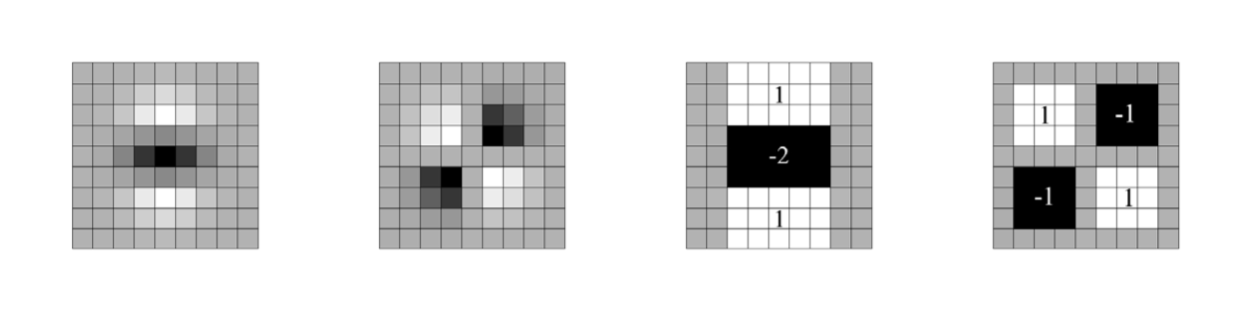
\includegraphics[width=0.7\textwidth]{l4template-master/images/boxfilters.png}
    \caption{The approximation of Gaussian second order partial derivatives using box filters \citep{Bay08}.}
    \label{boxfilters}
\end{figure}


Interest points at different scales are found by applying box filters of different sizes. The scale space is analyzed by up-scaling the filter size rather than iteratively reducing the image size. The following layers are obtained by filtering the image with gradually bigger masks, hence, for each new octave, the filter size increase is doubled. 

For the purpose of descriptor computation, the orientation of the point of interest must be determined. This is achieved by computing the Haar wavelet responses in horizontal and vertical directions around the point of interest. The dominant orientation is estimated by calculating a vector from the summation of all responses within a sliding orientation window covering a 60 degrees angle. Finally, the longest vector is selected which lends its orientation to the interest point. 

The descriptor is based on the sum of Haar wavelet responses. The region around the point is described by extracting a square region around the point of interest. The size of the region is directly proportional to the scale and is oriented along the orientation computed in the previous step. This region is split into smaller 4x4 square sub-regions and for each sub-region the Haar wavelet response is extracted. To offer more robustness for deformations, noise and translation the responses are weighted with a Gaussian. Finally, the responses are summed up over each sub-region to form a first set of entries to the feature vector. 

Bay et. all estimate that SURF outperforms SIFT by 4 times on average in computation time while not sacrificing in quality and robustness.


\subsection{Oriented FAST and rotated BRIEF}

Though SURF is on average faster than SIFT, it still imposes a large computational penalty. There are currently GPU implementations of both SURF and SIFT that aim to overcome this limitation but they are not suitable to use for real-time feature detection on low-powered devices that have limited computational capabilities. This has lead researchers to develop a suitable replacement for SIFT and SURF that has a similar matching quality while being more performant. 

One such alternative that builds on the FAST key-point detector and BRIEF descriptor, was developed by \citet{Rublee:2011:OEA:2355573.2356268} called Oriented FAST and rotated BRIEF (ORB).

Features from accelerated segment test (FAST) is a corner detection method. It uses a circle of 16 pixels around a point $p$. For each pixel in the circle the brightness is computed, and if more than half the pixels are either darker or brighter than $p$, then the point is selected as a key-point. While FAST features are widely used because of their computational properties, the FAST key-points are neither scale nor rotation invariant. To rectify this issue, in ORB, after the FAST points in the image are detected, a Harris corner measure is employed and the FAST key-points are ordered according to that measure, with top N points being selected. To make ORB features scale invariant, ORB employs a multi-scale image pyramid where for each level of the pyramid FAST features filtered by the Harris measure are produced. To make FAST features rotation invariant, the weighted intensity centroid of the patch around the detected feature is computed with orientation of the key-point being equal to the direction of the vector from the feature towards the centroid. 

\begin{figure}[ht]
    \centering
    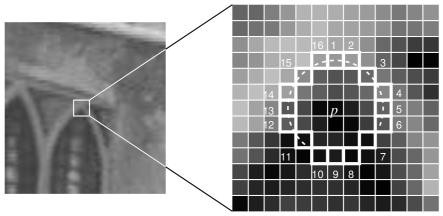
\includegraphics[width=0.7\textwidth]{l4template-master/images/FAST.jpg}
    \caption{12 point segment corner detection test \citep{fast}.}
    \label{fast}
\end{figure}

In ORB the descriptors are based on Binary Robust Independent Elementary Features (BRIEF) descriptors. To minimise the sensitivity of the descriptors to noise, the image is initially smoothed with a Gaussian kernel. Using the smoothed image, from a patch around a key-point with a set width and height, random pixel pairs are selected and intensity comparisons are done on them, assigning a value of 1 if the first pixel from the pair is brighter than the second pixel. For a 128-bit descriptor vector, this process is repeated 128 times for the same key-point. While this is fast to compute, BRIEF performs poorly with rotation. To allow BRIEF to be invariant to in-plane rotations of more than a few degrees, in ORB, a rotation matrix is computed using the orientation of the key-point and then the BRIEF descriptors are steered according to the orientation.

\citet{Karami} compared the performance of SURF and ORB against different kinds of transformations and deformations such as scaling, rotation, noise and fish eye distortions. It was shown that ORB is the fastest algorithm, however it is outperformed by SURF in matching quality in most scenarios. Similarly, \citet{Tareen2018ACA} shows that ORB outperforms SURF both in the number of features detected and the computational time but suffers in matching quality. This makes ORB suitable for applications where the decrease in computational time is more important than the small matching penalty compared to more accurate feature detectors. This the main reason why ORB is used in our application, where the speed requirements take priority over the matching quality. 


\section{Local Feature Matching}

\subsection{Matching strategies}
Matching descriptors from one set with the descriptors in a second set is usually performed by using two approaches: Brute Force Matching or applying a indexing structure. Brute Force Matcher is the simplest of the two. It functions by matching a descriptor from the first set with all the descriptors from the second set, returning the closest one based on distance measurement, such as Euclidean distance for SIFT and SURF and Hamming distance for ORB. While this is not efficient, it is guaranteed to return the best matches of the two sets. 

For the purpose of achieving a better matching performance, an indexing structure is devised. One of the most widely used indexing structures are the k-d trees, which are a class of multi-dimensional search trees. This matching algorithm is much faster for larger data sets, however, it is not guaranteed to return the best match, as it only returns the approximate nearest neighbours. 

Outlier rejection from the feature space is accomplished by comparing the distance value of the closest match to the distance value of the second-closest match. In his seminal paper, Lowe suggests to reject all the matches with a distance ratio greater than 0.8, which was the approach used in this project. 

In order to further eliminate the remaining error matches, a robust estimation method introduced by \citet{Fischler81} called Random Sample Consensus (RANSAC) is frequently used to to handle mapping features in the presence of outliers. 


\subsection{Homography}

Inlier correspondences between two images are found by computing the planar homography of the transformation. A homography, also known as plane projective transformation, is a 3 by 3 matrix \textit{H} that relates the transformation between corresponding image points as:
\begin{align}
x'=Hx 
\end{align}

Two images are related by a homography if and only if the image points correspond to the same planar surface in the real world and the images were acquired by rotating the camera about its optical axis. 

To compute the homography between two image pairs, RANSAC robust estimation is applied. For each iteration of the RANSAC algorithm:

\begin{enumerate}
    \item A random sample of 4 matches is selected and the homography \textit{H} is computed.
    \item The geometric image distance error for each match is calculated.
    \item The number of inliers from the number of matches for which the distance error is less than a threshold is computed.
    \item The homography with the largest number of inliers is selected.
    \item The least-squares homography estimate using all of the inliers is re-computed \citep{Torr2000}.
    
\end{enumerate}

%==================================================================================================================================
%==================================================================================================================================
%==================================================================================================================================
%==================================================================================================================================
%==================================================================================================================================

\section{Gaze Control}

One of the most important skills required for both biological organisms and artificial machines is the ability to direct the vision system towards a target. For humans, eye movements are split into mechanisms to either stabilize gaze or redirect gaze. The redirecting gaze mechanisms which are responsible for orienting the eyes to point to new locations are split into two classes: saccade movement and smooth pursuit movement. Saccades are rapid eye movements that allow us to quickly scan a visual scene and are characterised by quick, step-like rotations between fixation points, where the image of the visual target located at the periphery of the retina is moved to the center. Following each saccade, the eyes remain stationary at their new positions enabling the subsequent high-acuity detailed visual analysis at that location. The destinations of each saccade movement are selected by cognitive brain processes, with vision being dependent upon the information gathered during the pauses between saccades. Contrary to the rapid, step-like saccade movement, smooth pursuit eye movements slowly rotate the eyes in a linear fashion in order to keep a moving stimulus centered on the fovea.

The identification of relevant targets in the visual field is strongly interlinked with the behavioral and cognitive process called Attention that can be either overt attention or covert attention. The former category involves orienting the body, head and eyes to foveate a stimulus. The later is the act of shifting one's focus in the visual field without eye movements. A lot of research has been done for the purpose of understanding the selection process of spacial locations in the human attention with much evidence ( \citet{James1890}, \citet{Treissman1988}, \citet{Braun1998}, \citet{Itti2000} ) pointing towards a two-component framework for where in a visual scene attention is deployed. The most primitive one of the two, bottom-up mechanism, is an involuntary attention mechanism where the attention is grabbed by the most salient stimuli in our field of view with properties such as color, contrast and orientation being relevant. The top-down mechanism, on the other hand, occurs when we have a task in mind and direct the "spotlight of attention" under cognitive control. \citet{yarbus1967eye}, in his investigation of the correlation between the eye movement patterns and high-level cognitive factors, shows striking differences between eye-patterns based on the task the observer is instructed to perform while viewing a complex object. He concludes that the eyes fixate not on the most salient features of an image, but on those that provide the most information for the task at hand. 


\begin{figure}[ht]
    \centering
    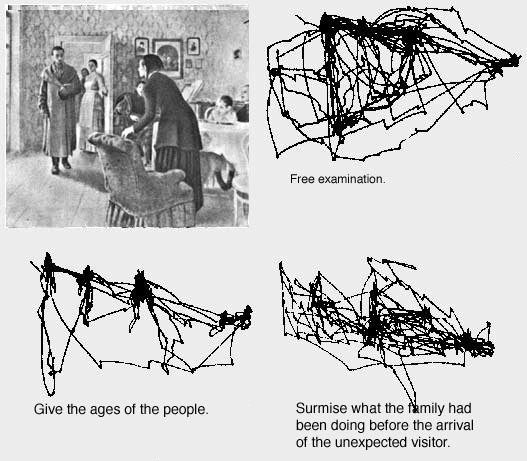
\includegraphics[width=0.75\textwidth]{l4template-master/images/Yarbus_The_Visitor.jpg}
    \caption{Yarbus' investigation of eye patterns based on task.}
    \label{Yarbus}
\end{figure}



Computational visual attention is a classic research area in computer vision and neuroscience, with numerous bottom-up and top-down models being proposed in literature. Because this work is concerned with stationary visual scenes where the only movement is performed by the PTZ Camera, we will focus on the bottom-up overt mechanisms using saccade movements. 


\citet{milanese1992} developed a bottom-up focus of attention system based on salient features extracted from the input image. In his approach, "conspicuity maps" that consist of interesting regions of the image are created from features that are distinct from their surroundings. These maps are then merged into a central saliency map, where sequences of attention shifts are generated based on the activity in the map. 

\citet{Fattah} used bottom-up saccade targeting as a means for gaze control, in which the attention system selects new saccade movements based on computed SIFT local features in the view of the cameras. To stop the camera from returning to locations that have already been attended, an inhibition of return (IOR) mechanism was implemented by maintaining a list of already  visited points. Similarly, \citet{Ozimek} selects fixation points for the software retina by populating a saliency map with SIFT features while maintaining an inhibition of return map where each fixation point is represented by amplified Gaussian spanning the retinal foveal region. By subtracting the IOR map from the saliency map, points that were previously visited are discarded. 




Unlike the works mentioned above where the saliency maps are populated with various hand-crafted features, the model developed by \citet{kruthiventi2015} predicts the pixel-wise saliency values for a given image using a fully convolutional neural network trained on eye-fixation data. 

While using CNNs such as DeepFix gives promising results, this work is based on the approaches of \cite{Fattah} and \cite{Ozimek} due to their simplicity and good performance. 






% \section{Gaze Control Original}

% One of the most important skills required for both biological organisms and artificial machines is the ability to direct the vision system towards a target. For humans, eye movements are split into mechanisms to either stabilize gaze or redirect gaze. The redirecting gaze mechanisms which are responsible for orienting the eyes to point to new locations are split into two classes: saccade movement and smooth pursuit movement. Saccades are rapid eye movements that allow us to quickly scan a visual scene and are characterised by quick, step-like rotations between fixation points, where the image of the visual target located at the periphery of the retina is moved to the center. Following each saccade, the eyes remain stationary at their new positions enabling the subsequent high-acuity detailed visual analysis at that location. The destinations of each saccade movement are selected by cognitive brain processes, with vision being dependent upon the information gathered during the pauses between saccades. Contrary to the rapid, step-like saccade movement, smooth pursuit eye movements slowly rotate the eyes in a linear fashion in order to keep a moving stimulus centered on the fovea. Because this work is focused on a stationary visual scene, where the only movement is done by the PTZ Camera, the gaze control will only be based on the saccade movement. 

% \citet{Fattah} used saccade targeting as a means for gaze control, in which the attention system selects new saccade movements based on computed SIFT local features in the view of the cameras. To stop the camera from returning to locations that have already been attended, an inhibition of return (IOR) mechanism was implemented by maintaining a list of already  visited points. Similarly, \citet{Ozimek} selects fixation points for the software retina by populating a saliency map with SIFT features while maintaining an inhibition of return map where each fixation point is represented by amplified Gaussian spanning the retinal foveal region. By subtracting the IOR map from the saliency map, points that were previously visited are discarded. These two approaches are an inspiration for the gaze control used in this paper. 

%==================================================================================================================================
%==================================================================================================================================
%==================================================================================================================================
%==================================================================================================================================
%==================================================================================================================================
%==================================================================================================================================
\chapter{Materials and Methods}

\textit{In this chapter we give an overview of the main hardware, frameworks and the software components we have used for this project.}




\section{Pan-Tilt-Zoom Camera} 

The camera used in this project is a network PTZ Camera manufactured by LEFTEK which is capable of remote directional and zoom controls. Even though cameras of this type were designed for surveillance applications only, we seek to analyse its suitability for collecting images for the purpose of training Neural Networks. The benefits of using this camera arise from it's relative cheap cost while providing a high resolution sensor and a wide angle lens both of which are necessary for capturing a high amount of details from a wide angle of view. In addition, its PTZ capabilities provide the possibility for capturing images from different angles and distances. 





\begin{figure}[ht]
    \centering
    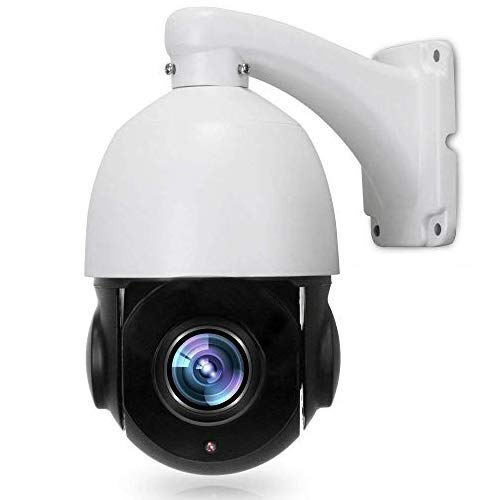
\includegraphics[width=0.3\textwidth]{l4template-master/images/ptzCamera.jpg}
    \caption{LEFTEK pan-tilt-zoom camera used in this project}
    \label{ptzCamera}
\end{figure}


This camera uses a number of protocols for controlling and video streaming purposes, the most important of them being: Hyper Text Transfer Protocol (HTTP), Real Time Streaming Protocol (RTSP) and Open Network Video Interface Forum (ONVIF). 


\section{OpenCV}

For image processing and extraction OpenCV (Open Source Computer Vision) framework is used. OpenCV is a cross-platform library aimed at real-time computer vision, image processing and machine learning written in C++. Even though OpenCV is mostly used in applications developed with C++, this project uses the Python OpenCV library that exposes the C++ functions through Python bindings.    

Beside basic image or video iInput/Output processing and displaying functionality, it has a set of built in complex algorithms for object and feature detection, Machine Learning, Computational Photography and others. In this paper, we are mostly focused on the features2D module that provides methods for 2D image feature and descriptor extractors such as SIFT, SURF and ORB.

Though there are other alternatives for image processing, none have the amount of built-in functionality OpenCV provides. Furthermore, because the ORB feature detection algorithm was developed by "OpenCV Labs", it solidified our decision of it being the framework of choice. 

\section{Graphical User Interface} \label{GUIbackground}

This project has inherited the Graphical User Interface (GUI) developed by \cite{JianwenZhou}. His work focused on integrating Ozimek's software retina into a tailored manual capture control interface capable of controlling the same camera used in this project. This GUI provides functionality for connecting to the camera and displaying a live view of the video stream. Additionally, it provides PTZ Controls which are implemented using the manufacturers proprietary HTML protocol. Finally, in terms of the software retina integration, it allows for the creation and saving of retinal transformed images and displaying the cortical and back-projected images.

In this project we seek to use this GUI as a baseline into which the Autonomous Capture component will be integrated, implementing the modifications necessary to fulfill this project's requirements. 

\begin{figure}[ht]
    \centering
    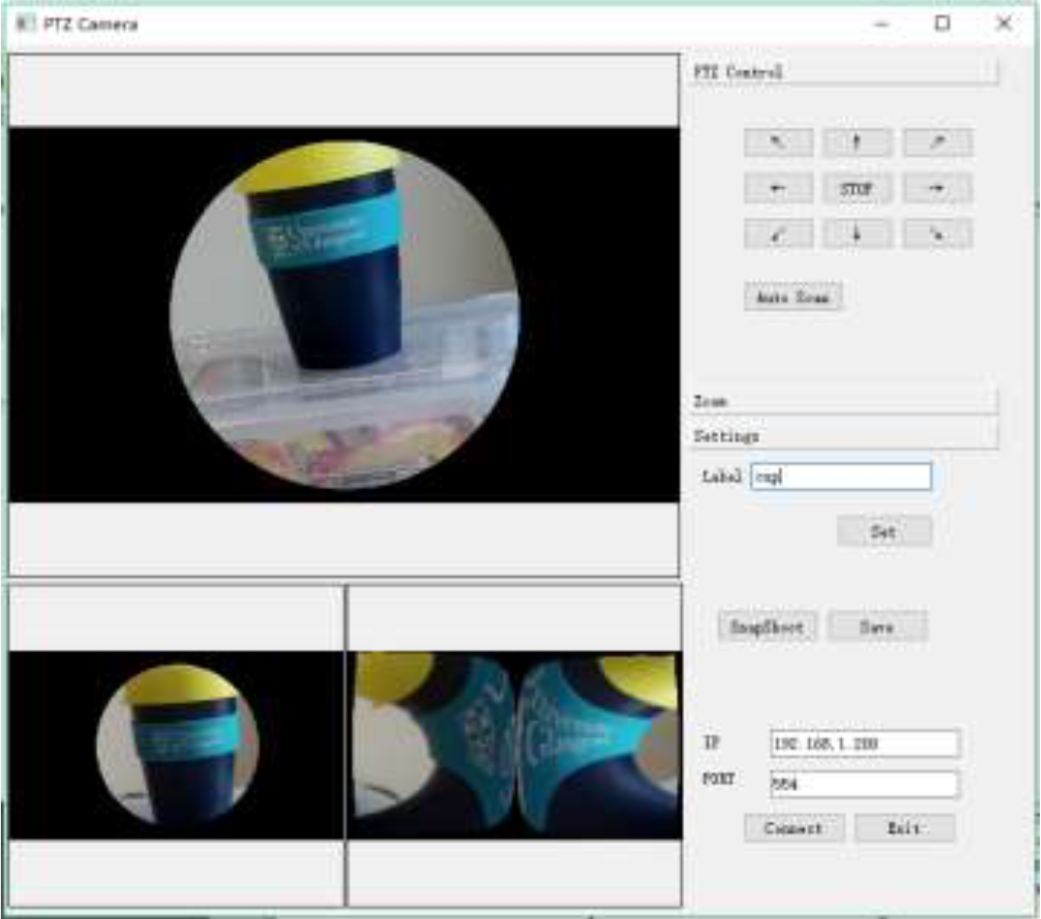
\includegraphics[width=0.6\textwidth]{l4template-master/images/old_gui_temp.png}
    \caption{Graphical User Interface developed by \cite{JianwenZhou}}
    \label{oldgui}
\end{figure}


%==================================================================================================================================
\chapter{Design and Implementation}

\textit{[PLACEHOLDER] In this chapter we describe in detail the implementation of our system. Firstly we discuss the benefits and the limitations of the ONVIF Protocol. Secondly we describe the architecture of the CameraController component and the implementation of the Gaze Control. Finally, the overall architecture and describe how all the components tie in together.}

\section{ONVIF Protocol}

One of the key requirements concerning the Controller component was for it to be implemented in a non-proprietary protocol. Because it is supported natively by the PTZ Camera, and because it is by far the most popular open standard for the interface of physical IP-based security products, \textit{Open Network Video Interface Forum} (ONVIF) was chosen as the protocol in which this component will be implemented. ONVIF defines a standard for how IP Camera products within the surveillance industry can communicate with each other. By implementing ONVIF, the same instructions such as initiating a video stream or moving the camera can be used for a big number of devices across different manufacturers. Therefore, if in the future there is a decision to replace the camera with a different model that supports the ONVIF protocol, it wont be necessary to rewrite the base implementation of the Controller. 


On the most basic level, in the ONVIF protocol, the functions exposed to the client are defined in Web Service Description Language (WSDL) files corresponding to each ONVIF service and the commands are sent via Simple Object Access Protocol (SOAP) requests. A developer can choose to implement the functions based on the WSDL files and by following the ONVIF Core Specification. In our application we make use of
\textbf{\textit{onvif-python}} library that offers an already implemented Access Point Interface(API) for these functions. Particularly, we utilise the ONVIF PTZ Service which defines the web service interface for configuration and operation pan-tilt-zoom controllers. 



One of the big limitations of the ONVIF protocol is that for a camera to be considered ONVIF compliant only the "core" specification must be implemented by the manufacturer. In the Move Operations specification there are defined 3 different PTZ move operations: AbsoluteMove, RelativeMove and ContinuousMove. In AbsoluteMove the position argument of this command specifies the absolute position to which the PTZ unit moves. In RelativeMove the translation argument specifies the difference from the current position to the position to which the PTZ device is instructed to move. In ContinuousMove, the velocity argument of this command specifies a signed speed value for the Pan, Tilt and Zoom.  Even though AbsoluteMove and RelativeMove offer an increased granularity and sensitivity for the move operations,  ContinousMove was the only one to be implemented by the manufacturer of the PTZ Camera used in this project. 

In ContinousMove operation the PTZ command is executed continuously until a stop command is received by the camera. While this is perfectly adequate for applications such as controlling the camera from a joystick or by pressing buttons, it is not very suitable for the level of control required in this project. 



\section{Controller Model}

In order to move the camera a certain amount of degrees or pixels using ContinousMove protocol, the movement of the camera must be timed. In the prototyping phase, the velocity of the camera for Pan and Tilt was estimated by timing how much time it takes to complete a full rotation in each dimension. However, it soon became clear that there are significant errors caused by the network lag, the time the camera takes to process the commands and the inaccuracies caused by the PTZ motors not having a consistent velocity in each direction. Because of this, the error of movement was very significant and the original implementation was not fit for purpose. To lessen the effect of these deficiencies, a new approach needed to be taken. 

One model that was considered was moving the camera with small adjustments towards the target while continuously checking if the target has been reached. This proved to be unfeasible because of the computational requirements needed to continuously match points from  different camera views as well as the slow movement that this will imply. Though this idea was discarded for the main Controller model, the basic functionality was reused to improve the accuracy of the movement. 


A different approach that was considered and finally adopted was to train a predictive model that takes into account the network delay, the signal lag and the physical inaccuracies of the camera and is capable of predictive a move time necessary to reach the specific target. The use of a Deep Neural Network was initially examined and discarded because of the unnecessary complexity and the amount of data required to train it. Finally, we decided upon using a a Linear Regression model.

During the data gathering process it also soon became clear that the camera does not only move differently based on it being a pan or tilt movement, it also has a different behavior when it moves in different horizontal and vertical directions. Due to this observation, it was decided to train 4 different models depending on the movement that is required: Pan-Left, Pan-Right, Tilt-Up and Tilt-Down.  

\subsection{Data Gathering}

For the purpose of training the Linear Regression model, it was necessary to gather data of the camera pixel displacement per time interval. To achieve this, PTZ Move requests were sent to the camera with the time interval increasing with steps of 10 milliseconds. Data was collected for each of 4 pan-tilt directions, with an average of 1100 data points collected for the tilt models. Owing to a bigger range of movement in the horizontal direction, for each of the pan models approximately 2600 points were collected. 


To calculate the pixel displacement between two image pairs, a process based on a feature detector needed to be used. While the quality of the feature detection and matching was a vital characteristic in the search of a suitable algorithm, because the pixel displacement for over 7400 image pairs needed to be computed, the computational requirements also needed to be considered. SURF was selected over SIFT as the feature detector algorithm of choice for this task because of its decreased computation time with a similar quality of matches as SIFT. 

\begin{figure}[ht]
    \centering
    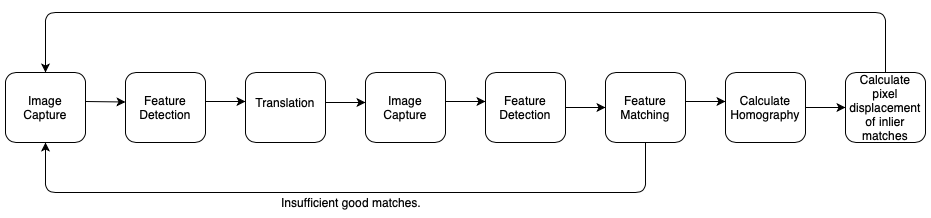
\includegraphics[width=1\textwidth]{l4template-master/images/dataGathering.png}
    \caption{Data Gathering Process}
    \label{datagathering}
\end{figure}


In the first part of the data gathering process, an image of an object is taken, and its features are detected using SURF. After the first set of features is computed, the camera translates for a specific amount of time and a second image is taken from which a second set of features is computed. To match the features between the two images, a choice needed to be made between the Brute Force Matcher (BFMatcher) and Fast Library for Approximate Nearest Neighbors (FLANN) based K-d tree algorithm. While FLANN has a lower computation time, the quality of the matches suffer as it is not guaranteed to produce the best matches. Because the quality of the matches was more important in this task than the increase in speed, BFMatcher was chosen as the matching algorithm. 

Once the potential matches were computed, the erroneous matches were removed in a two part process. Firstly, a part of the error matches were removed by applying Lowe's ratio test described in the Background section. In the second part of the process, the homography of the transformation between the two images is computed using RANSAC and the outlier matches are rejected. 

Finally, the pixel displacement of every inlier match is computed and the median value is calculated in order to minimise the influence of any remaining outliers that were not rejected previously.  


\subsection{Model Training}

After analysing the plotting the collected data, it became apparent that there is a linear relationship between the camera translation time and the pixel displacement. Therefore, it was decided to train simple linear models for the Camera Controller. 

Firstly, a suitable choice for a framework capable of training a machine learning predictive model needed to be made. \textit{Scikit-learn} is a very powerful, open source library based on SciPy, NumPy, and matplotlib. While there are numerous others Machine Learning frameworks, such as TensorFlow, Keras, PyTorch, which are more suitable for more complex Machine Learning models than a linear regression, Scikit-learn was chosen for the familiarity, simplicity of use and the great built in support for different kinds of generalized linear models.



Scikit-learn offers built in support for a big number of Linear Regression models, the most important of them being: Ordinary Least Squares, Lasso and Elastic Net. The later two are powerful techniques used for creating models in the presence of a very large number of features. The models apply regularisation techniques in order to penalise the magnitude of the less important features in the data set. Because the data used for training the models have only a feature per data point, the use of Lasso or Elastic Net was deemed unecessary and Ordinary Least Squares was used for training. 

Least Squares regression is the most common method for fitting a regression line. The underlying relationship between a dependent variable $y_{i}$ and an explanatory variable $x_{i}$ involving the error term $\epsilon_{i}$ can be described by:

\begin{align}
y = \alpha + \beta x_{i} + \epsilon _{i}
\end{align}


This method calculates the best-fitting line for the observed data by finding estimated values $ \hat{\alpha} $ and $\hat{\beta}$ which minimise the sum of the squares of the vertical deviations from each data point to the line. 

As part of the data preparation step, the outliers in the data were identified and removed by calculating the interquartile range (IQR) scores. IQR is is a measure of statistical dispersion, being equal to the difference between the upper and lower quartiles. While both variance and standard deviation are a measure of dispersion, IQR is much more robust to outliers. The data points that  were above 1.5 * IQR in the 3rd quartile and below the 1st quartile were removed from the data. 

Based on the collected data, there was no translation between the time intervals of 0.0-0.15 ms for Pan and 0.0-0.1 ms for Tilt, therefore the data points corresponding to those time intervals were removed from the training set, resulting in better fitted models with a variance score of 0.95 for Pan models and 0.98 for Tilt models. 


\begin{figure}[H]
  \begin{subfigure}[b]{0.5\textwidth}
    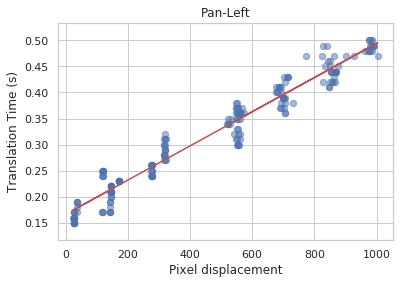
\includegraphics[width=\textwidth]{l4template-master/images/pan_left.png}
    \caption{Pan Left Model}
    \label{panleftmodel}
  \end{subfigure}
  %
  \begin{subfigure}[b]{0.5\textwidth}
    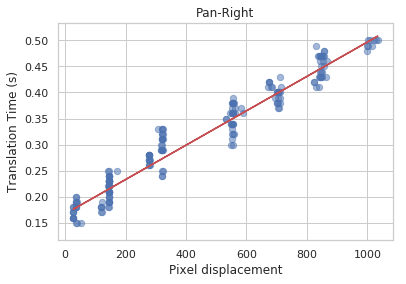
\includegraphics[width=\textwidth]{l4template-master/images/pan_right.png}
    \caption{Pan Right Model}
    \label{panrightmodel}
  \end{subfigure}
  \begin{subfigure}[b]{0.5\textwidth}
    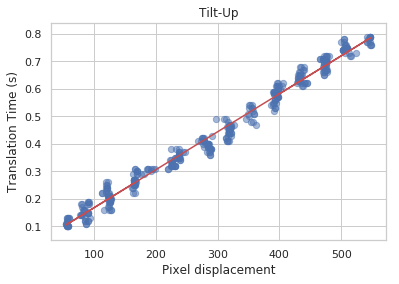
\includegraphics[width=\textwidth]{l4template-master/images/tilt_up.png}
    \caption{Tilt Up Model}
    \label{tiltup}
  \end{subfigure}
  \begin{subfigure}[b]{0.5\textwidth}
    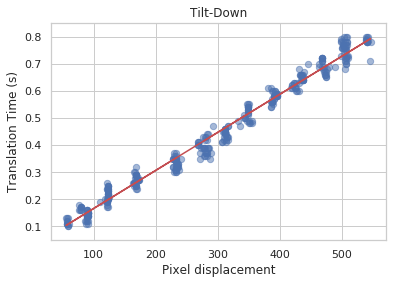
\includegraphics[width=\textwidth]{l4template-master/images/tilt_down.png}
    \caption{Tilt Down Model}
    \label{tiltdown}
  \end{subfigure}  
    
\end{figure}

The residual plots show that the difference between the predicted and real values are clustering around the lower y-axis digits. The data is also distributed on both sides of the y-axis, therefore the models don't tend to predict neither too low nor too high on average. However, one of the key requirements of a good residual plot is that there are no clear patterns on it. There is a clear quantisation of data observed in both the residual plots and in the Translation per Pixel displacement graphs. 


To remove the possibility of errors in the matching process and the homography computation to be the underlying reasons for this grouping of data points, for a series of image pairs the pixel displacement was manually determined and compared with the pixel displacement computed using the data gathering process described above. The results were consistent, having an average error of less than 10 pixels. Hence, no deficiency in the data gathering process has been found and the physical characteristics of the camera were determined to be the reason for this phenomenon. 

Based on the collected data and the models, for a 1920 by 1080 pixels image, the smallest translation for tilt and pan is 37 pixels and 57 pixels respectively.

\begin{figure}[H]
  \begin{subfigure}[b]{0.5\textwidth}
    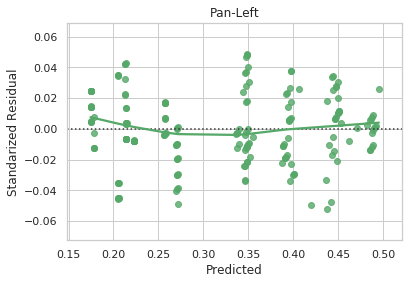
\includegraphics[width=\textwidth]{l4template-master/images/pan_left_residual.png}
    \caption{Pan Left Model Residual}
    \label{panleftmodelres}
  \end{subfigure}
  %
  \begin{subfigure}[b]{0.5\textwidth}
    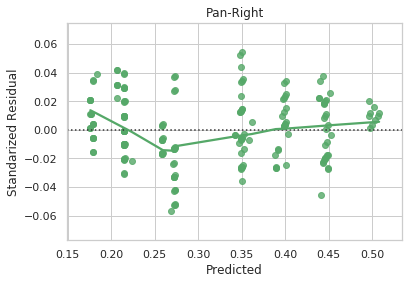
\includegraphics[width=\textwidth]{l4template-master/images/pan_right_residual.png}
    \caption{Pan Right Model Residual}
    \label{panrightmodelres}
  \end{subfigure}
  \begin{subfigure}[b]{0.5\textwidth}
    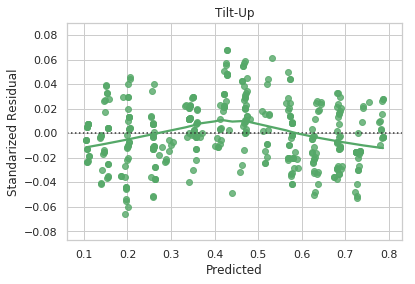
\includegraphics[width=\textwidth]{l4template-master/images/tilt_up_residual.png}
    \caption{Tilt Up Model Residual}
    \label{tiltupres}
  \end{subfigure}
  \begin{subfigure}[b]{0.5\textwidth}
    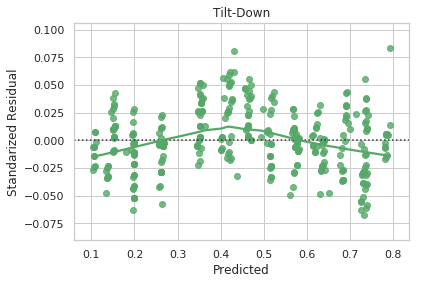
\includegraphics[width=\textwidth]{l4template-master/images/tilt_down_residual.png}
    \caption{Tilt Down Model}
    \label{tiltdownres}
  \end{subfigure}  
    
\end{figure}


\subsection{Controller Architecture}

After training a scikit-learn model, it is necessary to save the model for future use without having to retrain. This was achieved using Python's built-in persistence model called Pickle. Pickle is used for serializing and de-serializing Python object structures by converting Python object hierarchies into byte streams that can be saved to files.

\begin{figure}[ht]
    \centering
    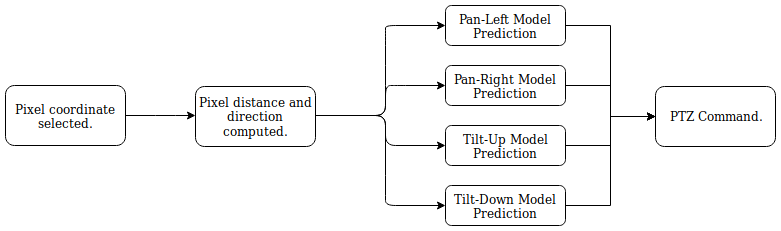
\includegraphics[width=1\textwidth]{l4template-master/images/Controller.png}
    \caption{Camera Controller}
    \label{controllerarchitecture}
\end{figure}

To direct the camera to a point on an object, the pixel coordinate on the image must be determined. Images in NumPy are multidimensional arrays, where each pixel value is stored as an element of the matrix that can be accessed by using NumPy's row-major-order indexing. Once the pixel coordinate has been selected, the Controller computes the direction and pixel distance of the point from image center. Depending on the direction, the suitable linear model is selected. The pixel displacement value is used as an input for that model with the output being the translation time prediction required for the camera to move in order to center on that specific point.

As mentioned above, the camera moves continuously from the moment a PTZ Command is received until the moment a Stop command is sent. This interval between the two commands is implemented using the built-in Python sleep() function used for pausing the execution of the program for a specific amount of time. Albeit this function is only accurate in the order of milliseconds and can be affected by the scheduling of other activities in the system and the implementation of the underlying Operating System's sleep function, it is perfectly acceptable for driving the camera with a similar expected performance across different Operating Systems.  

For the purpose of increasing the accuracy of the Camera movement, a simple retargeting algorithm was implemented. After a key point is selected and the camera translates to that point, local features are detected in the image after translation and the new position of the point is found. If the point is not found within the acceptable error margin from the image center, small incremental adjustments are performed using the smallest movement the camera is capable of until the point is within the acceptable distance. 

\begin{figure}[ht]
    \centering
    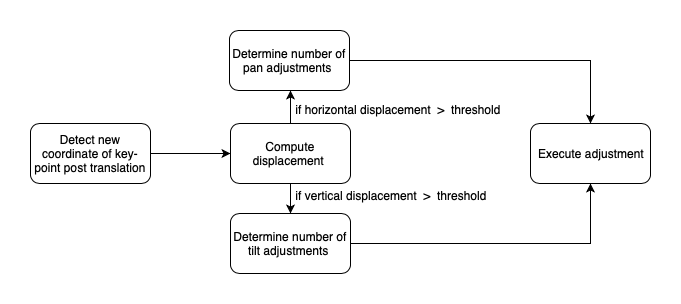
\includegraphics[width=1\textwidth]{l4template-master/images/retargeting2.png}
    \caption{Retargeting mechanism}
    \label{retargeting}
\end{figure}

% =======================================================================
\section{Gaze Control}



The gaze control mechanism in this work was inspired by the pre-attentive processing of visual information in the mammalian brain. In this subconscious process, an analysis of the visual information is performed on the entire visual field, detecting basic features of objects such as colors, contrasts and contours. After all this information is collected, the brain filters the information, selecting the information that has the highest saliency. 



For the purpose of detecting salient features on objects two different feature detectors were considered: SURF and ORB. In the initial stages of the development, OpenCV implementation of SURF was used for feature detection. Despite the fact that SURF is a much faster feature detector than SIFT, it proved to be too slow for real time feature detection. 

To make the final choice, the performance of SURF and ORB was compared. For the same image, ORB detected 11589 features with an average computation time of 0.01747 seconds. SURF, on the other hand, detected 5780 features in 0.15748 seconds, which corresponds to approximately 10 times decrease in speed for half the amount of features detected. Because computational time was of an essence in this application, ORB was selected for the final implementation. 


\begin{figure}[ht]
  \begin{subfigure}[b]{0.49\textwidth}
    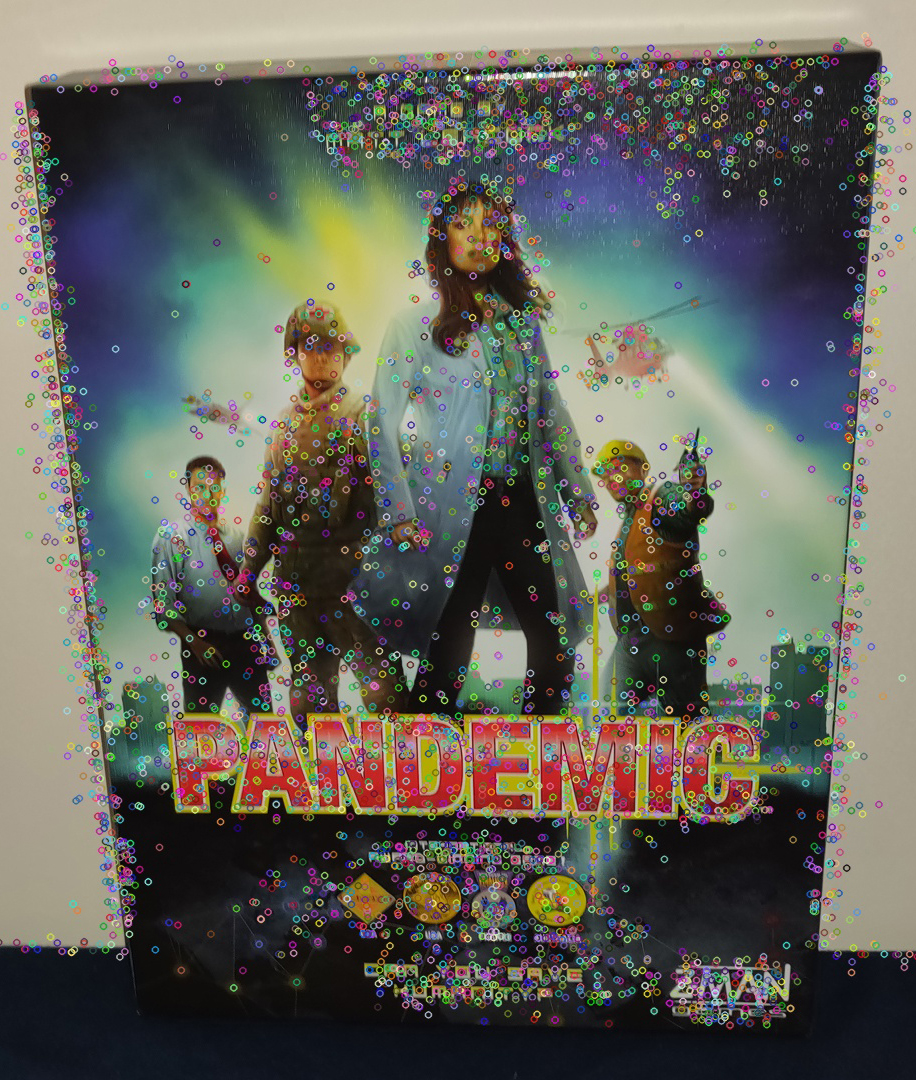
\includegraphics[width=\textwidth]{l4template-master/images/surf_keypoints_example.jpg}
    \caption{SURF features.}
    \label{surffeatures}
  \end{subfigure}
  %
  \begin{subfigure}[b]{0.49\textwidth}
    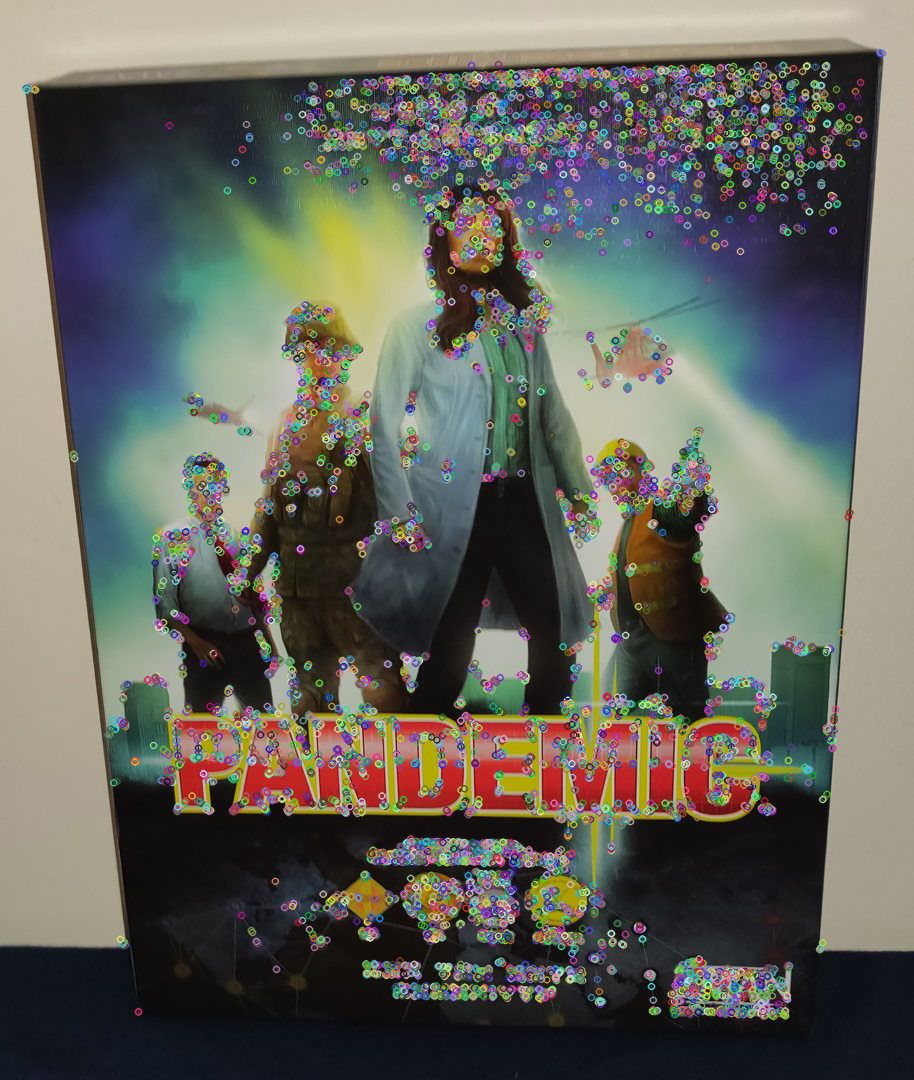
\includegraphics[width=\textwidth]{l4template-master/images/orb_keypoints_example.jpg}
    \caption{ORB features. }
    \label{orbfeatures}
  \end{subfigure}
  \caption{Comparison of features detected by SURF and ORB}
  \label{features}

\end{figure}

Once the local features of an object are computed, the key points are sorted and the most salient points are selected. Based on the work of \citet{RyanWong}, there are two factors that affect the choice of the focal point. The first factor is the intrinsic ORB keypoint response value which defines how strong the keypoint is. The second factor is the distance on the horizontal axis of the keypoint from the center of the image. Assigning a higher priority to keypoints further away from the image center allows for the exploration of other areas of the image without the same region of the object being explored continuously. The horizontal distance is normalised between 0 and 1 by dividing it with half the image width. 


Using equation \ref{ranking}, the new key-point rank, $kp{rank}$ is calculated assigning higher weight to strong key-points further away from origin.


\begin{equation}\label{ranking}
 kp_{rank} = \frac{(kp_{loc} - origin_{loc})}{(cort_{width}/2)} \times kp_{response}
\end{equation}

 
To avoid visiting the same regions of the object, an Inhibition of Return mechanism is implemented by saving in memory the key-points that were previously selected. Once the $kp{rank}$ is calculated for every key-point, they are sorted by their new rank. Before a new focal point is selected, the list of new key-points is matched with the IOR list and the matched key-points are discarded. 

Very frequently there are small regions with tightly packed key-points, which is also observed in figure \ref{features}. To avoid visiting key-points which are in the immediate proximity of a previously selected key-point, a circular mask around the coordinates of the key-point is applied, and the key-points withing the mask are detected and added to the IOR list. 

Once the already visited focal points are discarded, the remaining key-point with the highest value is selected. 

An important consideration for the Gaze Control is the speed of selection of focal points from the current view. In our implementation
the process of matching of already visited key-points with the new set of key-points as part of the Inhibition of Return mechanism is the bottleneck. The computation time becoming significant when a large area of an object is already explored and the IOR list   is populated with a significant number of key-points. To minimise the matching time, FLANN algorithm is used. 


\section{Supporting Modules}


\subsection{Retina}
We are using the RetinaVision module developed by \citet{Ozimek} using the 50000 node retina with a retina radius of 465 pixels. Ozimek provides another retina with 8000 nodes however it was deemed to be unsuitable due to a much smaller radius. 

At the start up of the application the files containing the retinal node locations and the receptive field kernes and the equivalent cortical files are loaded. The retina is then prepared by pre-computing the Gaussian normalization image. 

To increase the speed of computation of image vectors, the GPU accelerated CUDA codes were enabled, resulting in a significant increase in speed over using just the CPU. 


\subsection{DataStore}

For storing the data captured by the Autonomous Capture activity, the DataStore module developed by \citet{JianwenZhou} is used. To decrease the storage footprint of the captured data-sets only the generated imagevector and its metadata is saved to hard-drive.

The metadata of the imagevector consists of 4 different fields: "label", "fixationy", "fixationx" and "retinatype". The first field is used to identify different objects, in most cases the "label" field being the name of class the object is part of. The horizontal and vertical fixation coordinates are stored in "fixationy" and "fixationx" respectively. Finally, the last field corresponds to how many nodes the retina used to generate the imagevector has. To store the imagevector along with its metadata, Hierarchical Data Format (HDF5) is used which is a data format designed to easily store and manipulate big data-sets of multi-dimensional numerical data. 

No modifications were needed to integrate this module into our our project. 



\subsection{KeypointsUtility}

Because the same functions were being reused from the beginning of the development in different components, it was decided to separate all the logic related to local features into a separate module which can be imported and used by every other class in this project.

This module houses all the methods necessary for detecting local features, matching them and computing homography estimations in order to remove the erroneous matches. By separating the logic, the code repetition was reduced and the maintainability of the code was improved. 

\section{AutonomousCapture}


\begin{figure}[H]
    \centering
    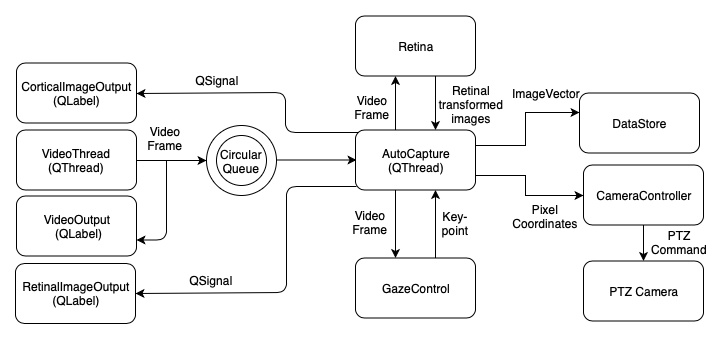
\includegraphics[width=1\textwidth]{l4template-master/images/overallarchitecture.png}
    \caption{The overall architecture of the program}
    \label{overallarchitecture}
\end{figure}


This is the main class of the application, which interlinks the GUI with the Gaze Control, the Camera Controller and the Image-vector saving functionality. 


To avoid the GUI freezing while the camera is capturing images and to allow for the dynamic display of the generated Cortical and Retinal images, AutoCapture has been implemented as a QThread. QThread objects manage one thread of control within PyQt programs. They are wrappers over native platform threads that provide additional functionality such as asynchronous signals, slots and event loops. It is possible to use native Python threads in PyQt application, but in order to interact with the main Qt thread, QThreads must be used.

\subsection{Image Capture}

In the initial stages of the development, images were captured using the OpenCV VideoCapture class which provides an API for video capturing from video files, image sequences or cameras. This object can be created by passing either the file path of the video file or the address of the network camera. One limitation of it is that if the connection is kept open, the video frames populate a buffer if they are not queried in a timely manner. As a temporary workaround, a new connection to the camera was being created every time a picture needed to be captured. This proved to be far too computationally expensive and a significant bottleneck for the performance of the application. 

A solution to this problem is to reuse the video frames captured by the VideoThread used for displaying camera's video stream which creates a VideoCapture object and keeps the connection open for the entire duration of the application. Because the video frames need to be shared between two different threads, a thread safe data structure needs to be used. Furthermore, because AutonomousCapture thread consumes the video frames slower than the VideoThread produces them, a similar buffering issue as the one described above can arise. 

The data structure chosen for this task is the \textit{Deque} which is a generalization of stacks and queue that supports thread-safe, memory efficient appends and pops with a performance of O(1). When a maximum length is specified and the dequeue becomes full, the same number of items are discarded from one end as the number of items appended to the other end. A small-sized dequeue is used to guarantee that the frames the AutoCapture thread consumes are as recent as possible. This proved to work very well, having good performance without having the need to re-create computationally expensive connections to the camera. 

\subsection{Inter-thread communication}

In a PyQt application, functions and methods are executed in response to events that can be generated by users interacting with widgets or by other QThreads. Each QThread can emit a 'signal' which is connected to a Python function defined in the main thread. 

In AutoCapture 3 signals are defined. Two of the signals are responsible for transferring the generated cortical and back-projected images in order for them to be displayed dynamically. The last signal is used to communicate to the main thread that AutonomousCapture has finished running.

To finish the execution of AutonomousCapture thread prematurely when the user presses on the Stop button, the main thread keeps a reference to the worker thread and changes a boolean flag inside the thread. This ensures that the thread finishes it's execution in a orderly manner after the previously computed imagevectors are saved to the hard-drive. 







\section{GUI Modifications}

As mentioned in Section \ref{GUIbackground} the Graphical User Interface used in this project is a modified GUI developed by \citet{JianwenZhou} for his Manual Capture Control interface. This GUI is developed using the PyQt5 framework which is a set of Python bindings for the Qt framework used for creating cross-platform graphical user interfaces. 

\begin{figure}[h]
    \centering
    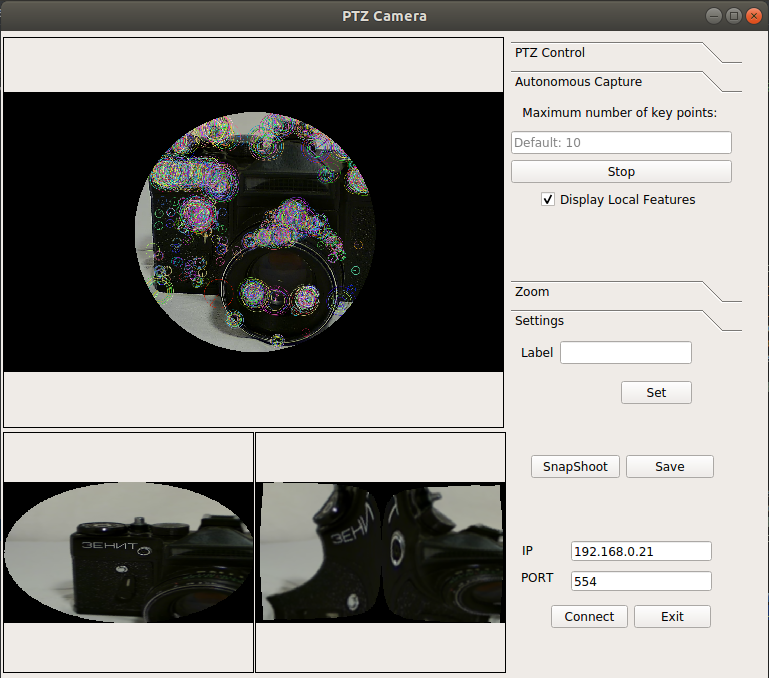
\includegraphics[width=0.7\textwidth]{l4template-master/images/guimodified.png}
    \caption{Modified GUI showing the controls used for launching the AutonomousCapture functionality.}
    \label{modifiedgui}
\end{figure}

To integrate my components into the GUI, a set of new controls needed to be developed. The original GUI uses a Toolbox container to separate different functionality by tabs, with the PTZ Control, Zoom and Settings having a separate tab. 

An additional tab that houses the controls needed for the Autonomous Capture was created with 3 different widgets inside. The first widget allows the user to enter the maximum number of key-points that they want the camera to detect and visit. The second widget is a push button that starts the AutonomousCapture thread. Once the AutonomousCapture is started, the button changes its text from "Start" to "Stop", and is used to stop the camera from capturing more images.   Finally, a check-box is provided which allows the user to choose if they want the local features detected in real time to be displayed in the video stream. 

In the original implementation there is no error handling for the processing of data given by the user in the input boxes and there are issues with the connection functionality. One such example being the application crashing if the user does not input an IP address or PORT number before they click Connect. 
These limitations have been fixed and the error handling was improved.  









\chapter{Evaluation and Analysis}

\section{Testing Environment}
\subsection{Hardware}

The performance of both the software retina and the detection of feature points is strongly dependent on the hardware used. To keep results consistent, for every test the hardware used both in the development and the subsequent evaluation has this specification:

\begin{table}[H]
\centering
\begin{tabular}{l|l}
Operating System & Ubuntu\\ \hline
GPU & NVIDIA GTX 970 \\ \hline
CPU & Intel Core i5-4690 CPU @ 3.50GHz\\ \hline
Camera Model & LEFTEK MY-57S-UB \\ \hline
Video Resolution & 1960x1080 pixels \\ \hline
Software Retina & 5000 nodes

\end{tabular}
\end{table}


\subsection{Materials}
For the experiments, six scenes with a different object in each scene is created. Objects have been selected to represent different sizes, shapes and textures. Because the application can't isolate the objects from a cluttered environment, in each scene a white sheet is used to create a contrast between the object and the background.

\begin{figure}[H]
    \centering % <-- added
\begin{subfigure}{0.20\textwidth}
  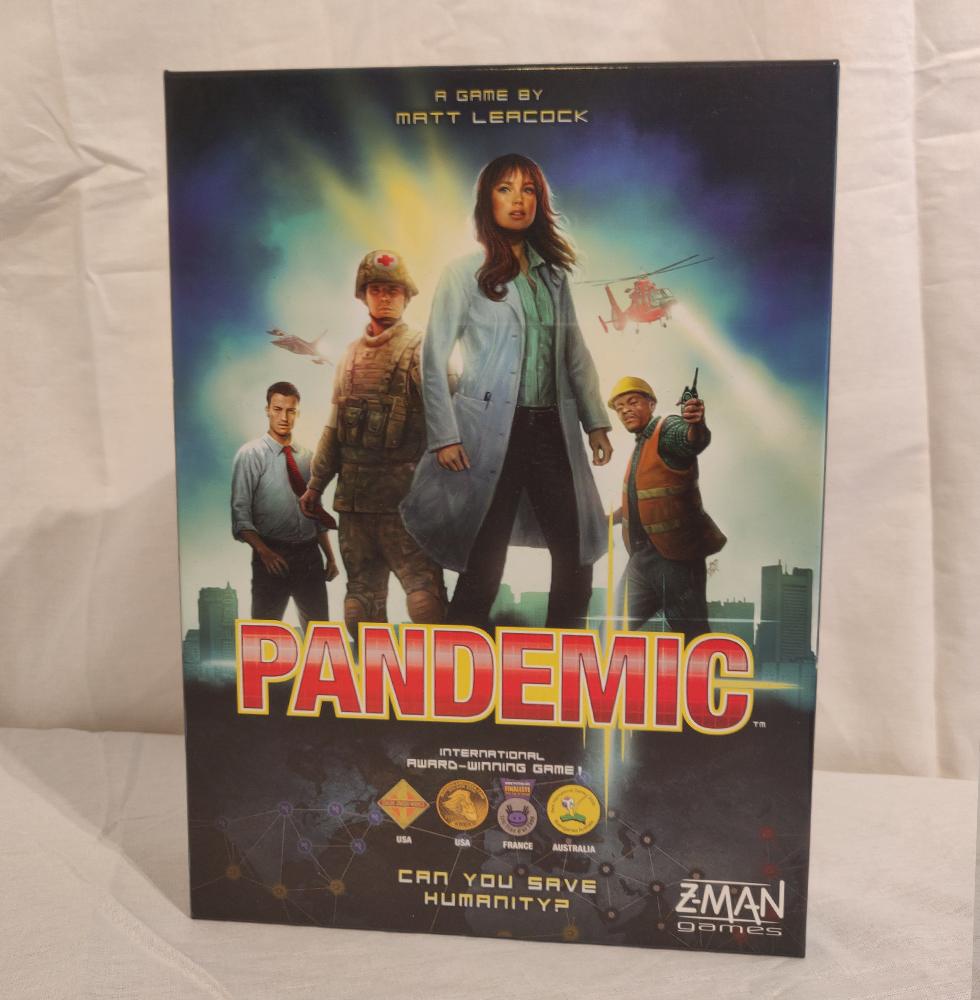
\includegraphics[width=\linewidth]{l4template-master/images/board_game.png}
  \caption{Board game}
  \label{boardgame}
\end{subfigure}\hfil % <-- added
\begin{subfigure}{0.20\textwidth}
  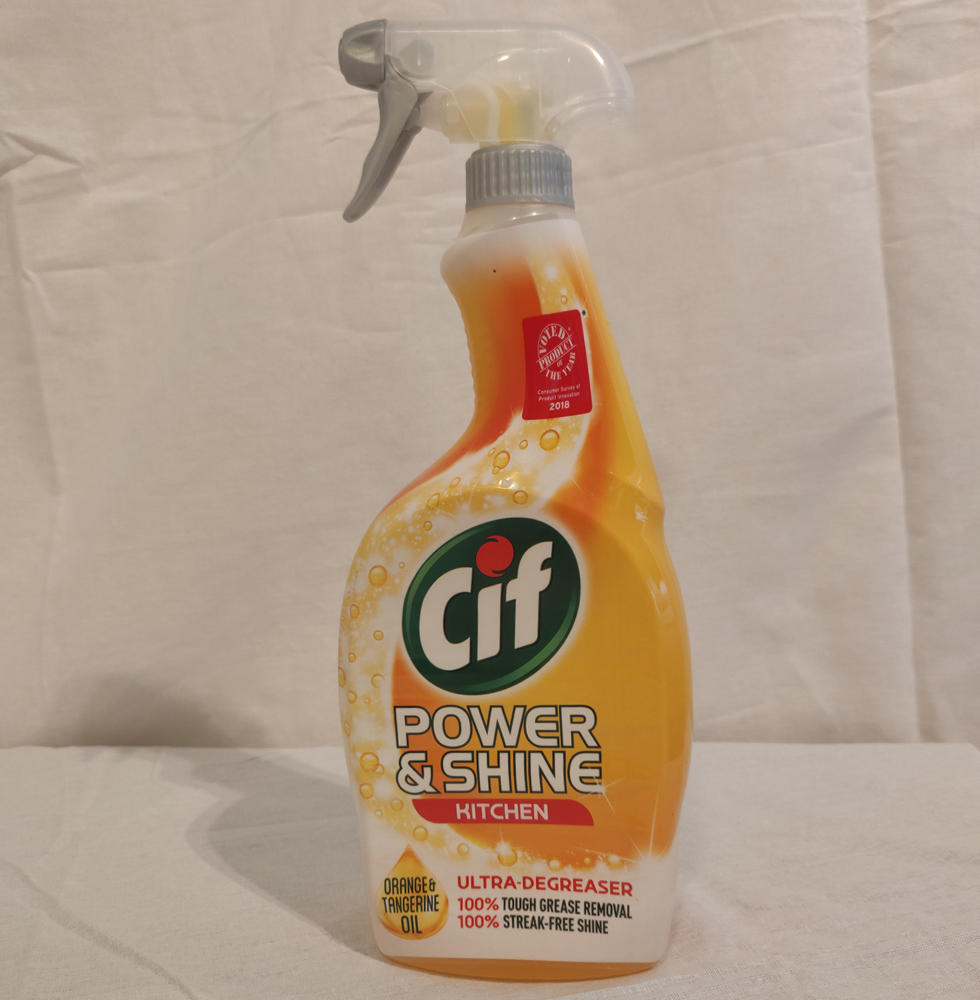
\includegraphics[width=\linewidth]{l4template-master/images/cif.png}
  \caption{Cleaning product.}
  \label{cleaningproduct}
\end{subfigure}\hfil % <-- added
\begin{subfigure}{0.20\textwidth}
  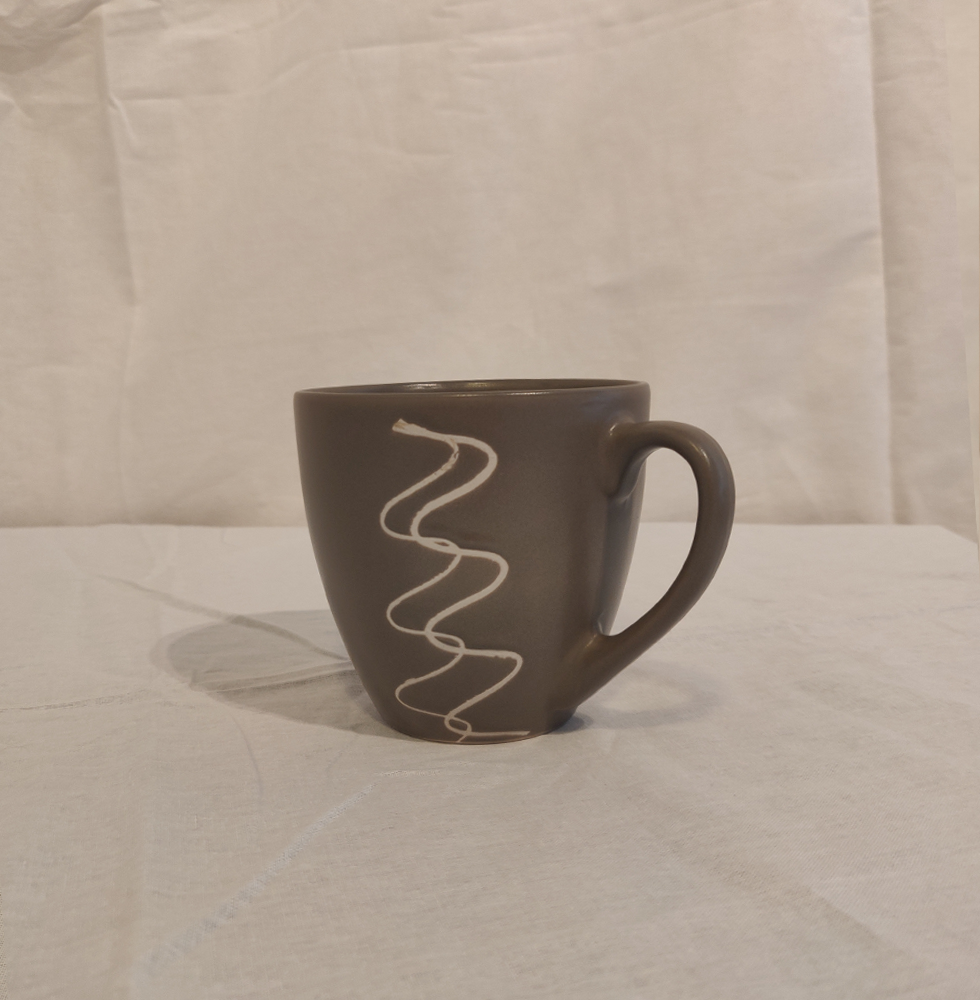
\includegraphics[width=\linewidth]{l4template-master/images/cup.png}
  \caption{Tea cup.}
  \label{teacup}
\end{subfigure}

\medskip
\begin{subfigure}{0.20\textwidth}
  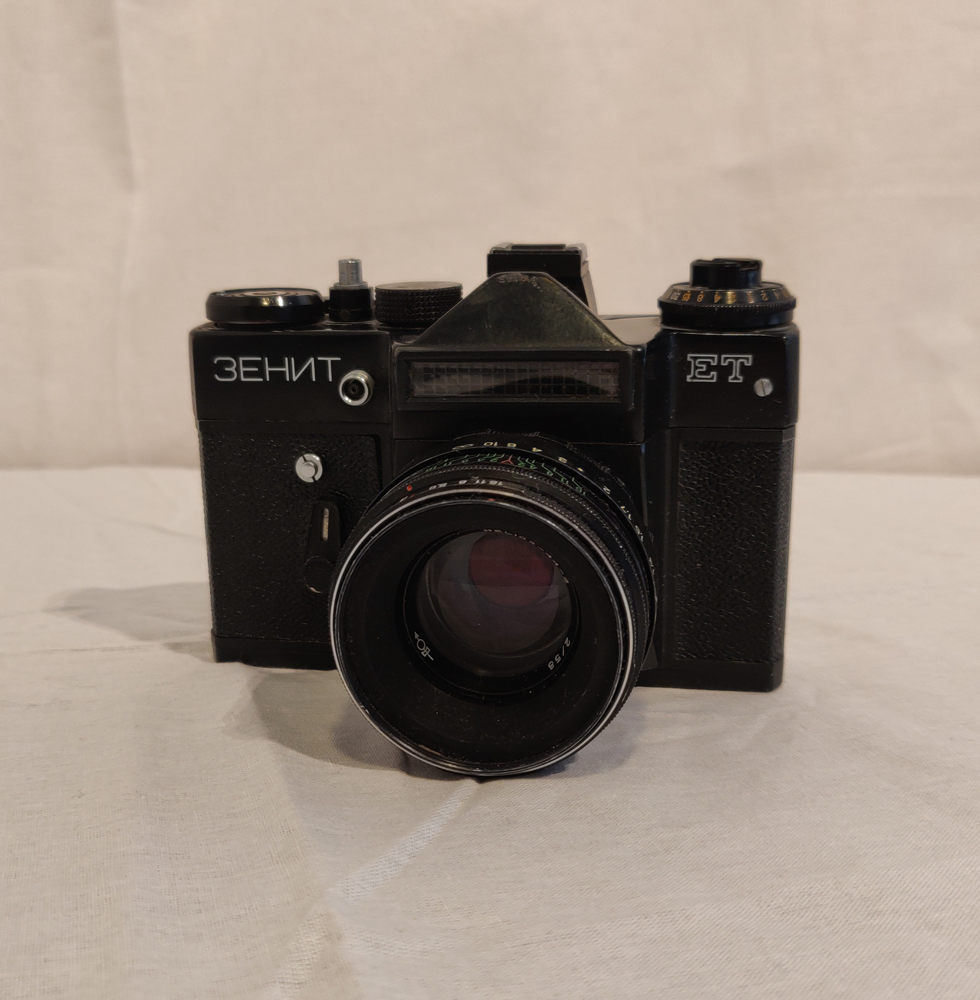
\includegraphics[width=\linewidth]{l4template-master/images/camera.png}
  \caption{Film camera.}
  \label{fig:4}
\end{subfigure}\hfil % <-- added
\begin{subfigure}{0.20\textwidth}
  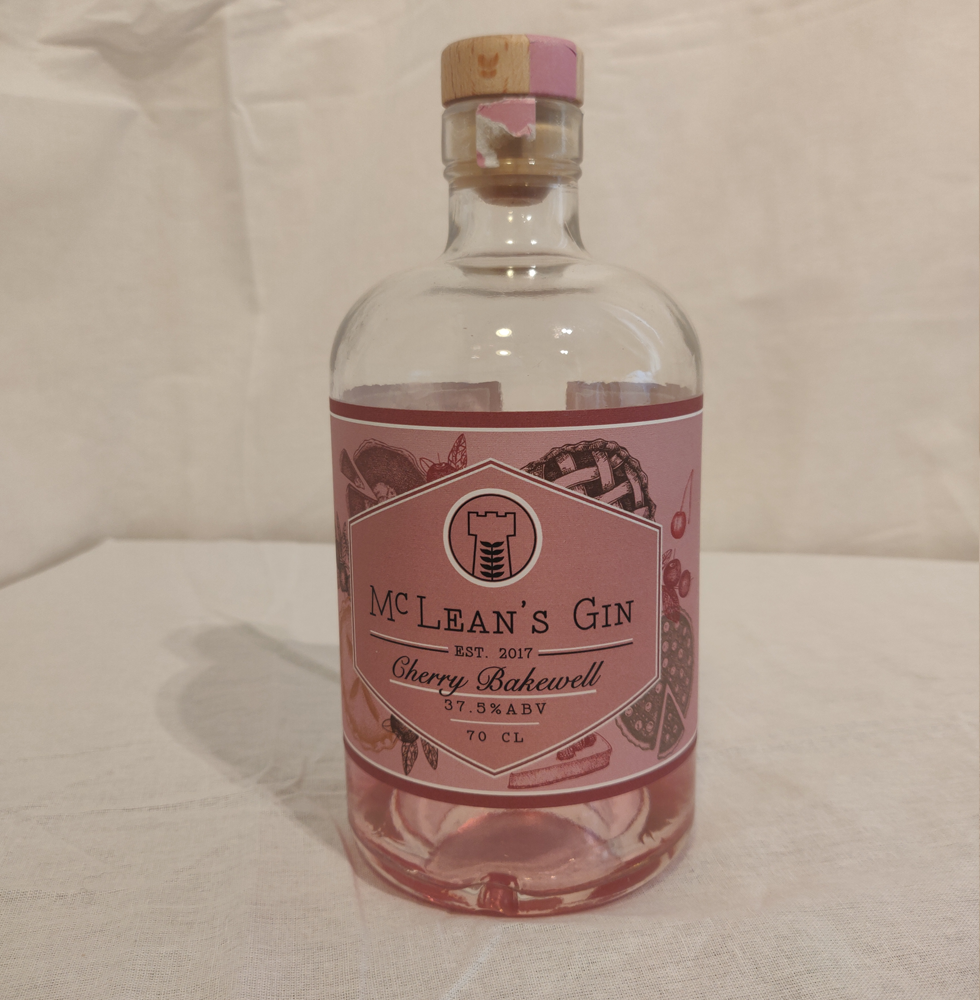
\includegraphics[width=\linewidth]{l4template-master/images/gin.png}
  \caption{Bottle of gin}
  \label{ginbottle}
\end{subfigure}\hfil % <-- added
\begin{subfigure}{0.20\textwidth}
  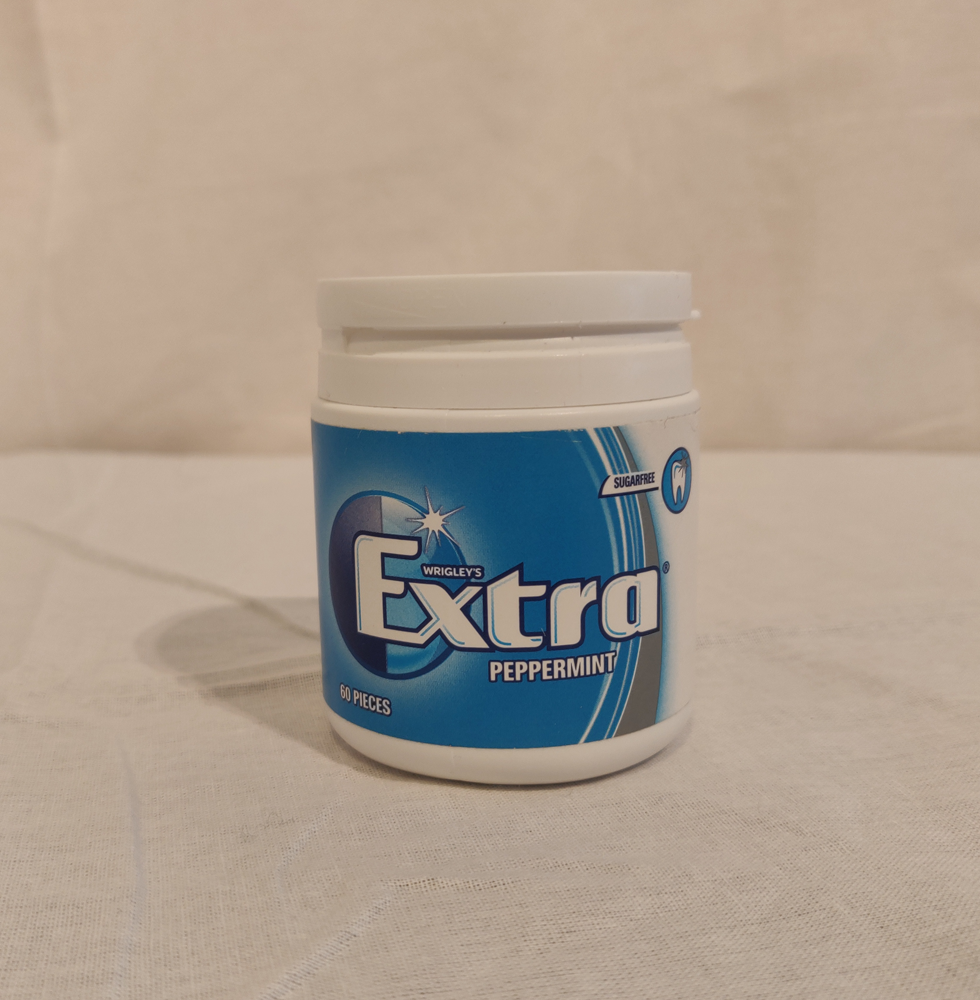
\includegraphics[width=\linewidth]{l4template-master/images/chewing_gum.png}
  \caption{Pack of chewing gum.}
  \label{chewinggum}
\end{subfigure}
\caption{Selection of objects used in the evaluation.}
\label{objects}
\end{figure}





\section{Controller Model Evaluation}
The first set of experiments concerns the verification of the Camera Controller and the Linear Regression models. The main aim is to measure the accuracy and reliability of the Camera Controller when used in a real-case scenario. For these results to be positive, the movement should be accurate enough for a focal point to be within the fovea's field of view which has a radius of approximately 45 pixels. The second aim is to compare the effectiveness of the Camera Controller with and without the re-targeting algorithm. 






\begin{itemize}
    \item \textbf{Setup:} Each object from Figure \ref{objects} is placed in front of the camera at a distance inversely proportional to their size. 
    
    \item \textbf{Methodology:} A set of feature points are detected. To select strong features with a good spread of distances from the image center, out of 10 strongest features detected a random feature is selected from the set. The pixel coordinates of the key-point is passed to the CameraController, which centers the camera on that area. Afterwards, the coordinates of the matching key point post translation is determined and the new displacement from the image center is calculated. For each scene from Figure \ref{objects} data from 200 translations was gathered. Finally, the re-targeting algorithm was removed and the experiment repeated in order to test it's effectiveness.
    
    
    \item \textbf{Results:}  From Figure \ref{meanerror} we can observe that for all 6 scenes, the mean pan error is under 55 pixels which in a 1080x1920 image corresponds to a error of approximately 3\%. Furthermore, in 4 out of the 6 scenes the mean error is smaller than the foveas' radius. This result is drastically improved when the re-targeting algorithm is used, decreasing the mean error to under 27 pixels or 1.4\%. Tilt on the other hand has much better results than pan when the re-targeting algorithm is not used, having a mean error of less than 20 pixels in all 6 scenes, corresponding to less than 2 \% error. There is no improvement when the re-targeting algorithm is used with a difference of +- 2 pixels between these two modes. 
    
\end{itemize}

Based on the limitations of the camera, the results described above are positive. Though in 2 out of 6 cases the horizontal error is slightly above the threshold, it is lowered when the re-targeting algorithm is used to make incremental adjustments after the initial movement finishes. The accuracy of the vertical movement is very good both with and without adjustments. This data justifies the use of the linear regression models and the re-targeting algorithm as in most cases the focal points will be comfortably within the radius of the fovea, which is the main requirement of this project. One interesting observation is the data from the coffee cup scene does not follow the same trend as the rest of the data. In the rest of the 5 scenes the magnitude of the error using the re-targeting algorithm is proportional to the error without the adjustments but this is not the case for the cup scene. This can be explained by the key-points being mismatched because of the complicated texture of the cup which in turn can corrupt the data. This shows a limitation of the re-targeting algorithm because it relies on the correct matching of key-points which is not a guarantee in this application. 





\begin{figure}[H]
  \centering
  \begin{subfigure}[b]{0.8\textwidth}
    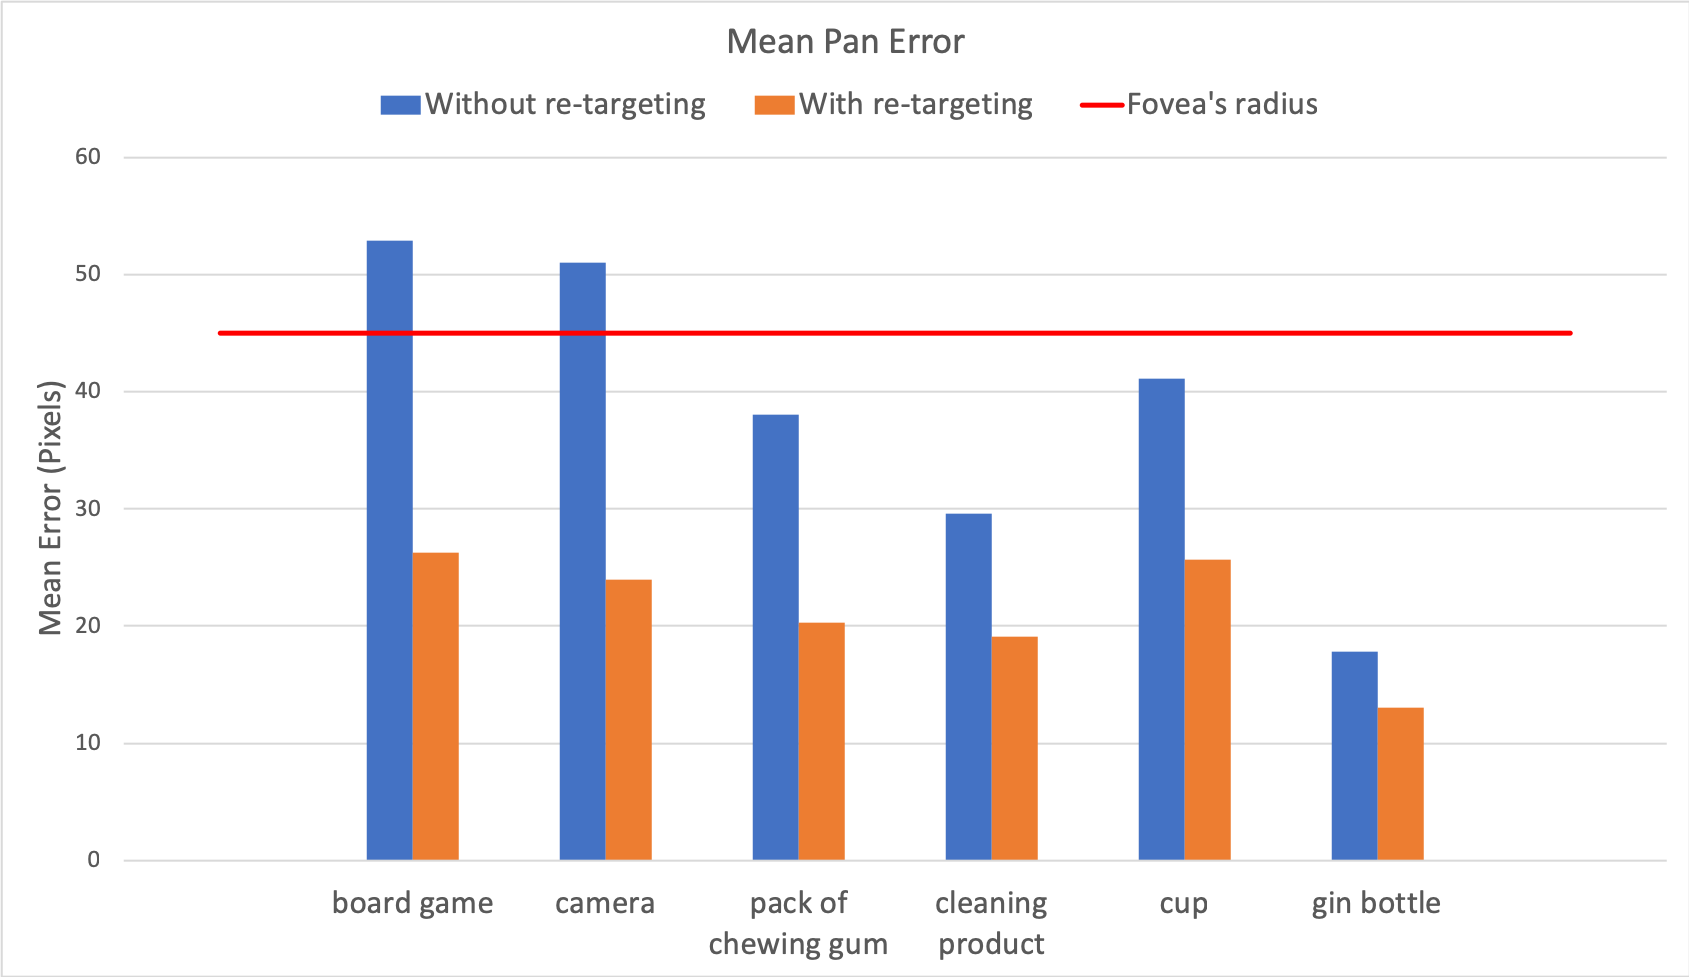
\includegraphics[width=\textwidth]{l4template-master/mean_pan_error.png}
    \caption{Pan error.}
    \label{panerror}
  \end{subfigure}
  
  \begin{subfigure}[b]{0.8\textwidth}
    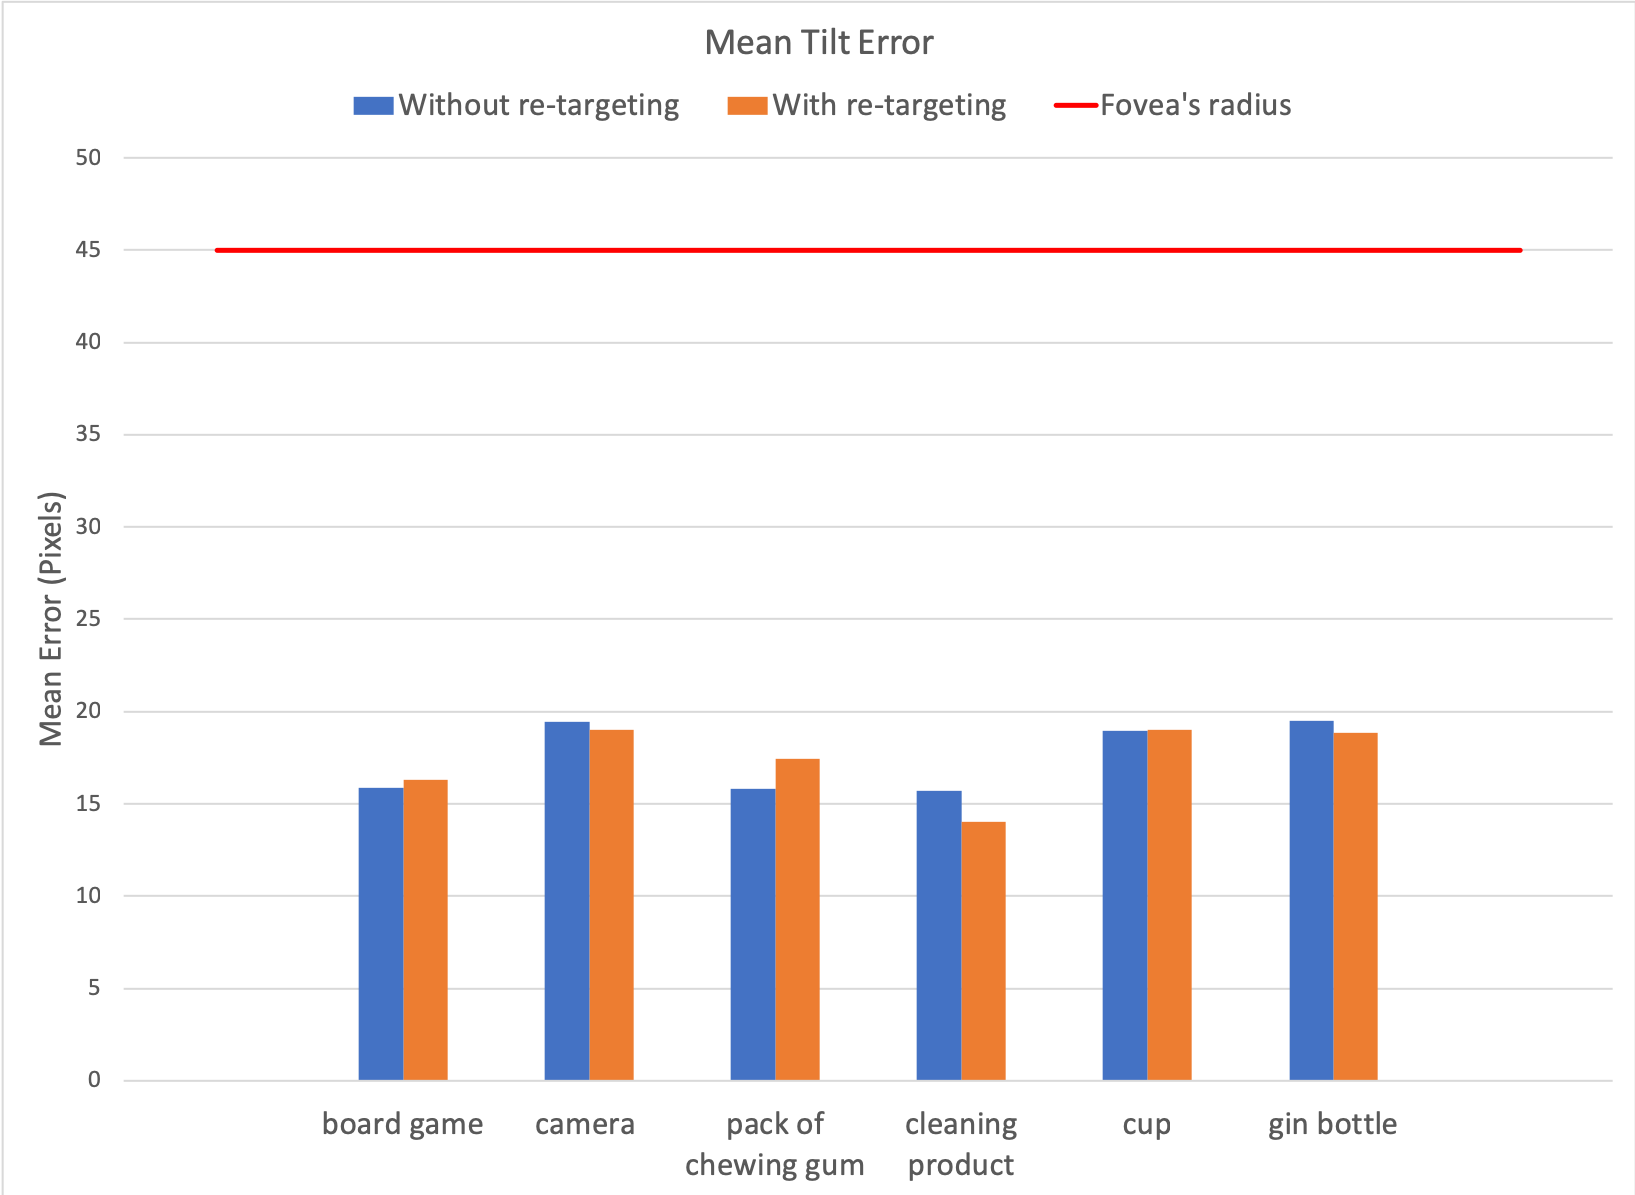
\includegraphics[width=\textwidth]{l4template-master/mean_tilt_error.png}
    \caption{Tilt error.}
    \label{tilterror}
  \end{subfigure}
  
  


\caption{Mean translation error in pixels.}
\label{meanerror}
\end{figure}

\section{Gaze Control Evaluation}
\subsection{Performance}

The second set of experiments concerns the performance of the Gaze Control algorithm. The intention behind this experiment is to evaluate the computational time for a focal point to be detected. Because the performance of the Gaze Control mechanism algorithm varies depending on how many features are in the field of view and of how many local feature were already visited, the scenes with the highest number of features needed to be selected.
\begin{itemize}
    \item \textbf{Set-up:} The scenes in Figures \ref{boardgame}, \ref{cleaningproduct} and \ref{ginbottle} were recreated in front of the camera. 
    \item \textbf{Methodology:} 20 key-points are detected and the computational time required to select the focal points is registered. Afterwards the mean value of each focal point across the 3 scenes is calculated. 
    \item \textbf{Results:}
\end{itemize}





\subsection{Gaze Control target selection}

This set of experiments concerns the quality of the selected targets by the Gaze Control algorithm. It is difficult to validate a Gaze Control algorithm because there is no benchmark it can be compared to. In these experiments a visual analysis of the Gaze Control target selection is performed both in a static setting where the image doesnt change and in the dynamic setting where the camera moves around. The most obvious thing that can be visually validated is the Inhibition of Return mechanism where the performance of it can be validated by seeing if the same areas are visited all over again and if the points are spread over the object or are in a confined area.  

\begin{itemize}
    \item In the first part of the experiment, a static image of the object in Figure \ref{boardgame} is used. In second part of the experiment, the scene is 
\end{itemize}






\section{Overall Evaluation}


\chapter{Conclusion}









\bibliographystyle{abbrvnat}

\bibliography{l4proj}

\end{document}
